\documentclass[11pt,a4paper]{article}

\usepackage{Rapport_Final} %% cibler doc/modules/

\usepackage{listings}
\usepackage{color}


\usepackage{fancyhdr}
\fancypagestyle{basdepage}{
\fancyhead{}
\fancyfoot{} % clear all footer fields
\fancyfoot[C]{Stage Lip6 : Amélioration de la réactivité des réseaux p2p pour les MMOGs (\thepage)}
\renewcommand{\headrulewidth}{0pt}
\renewcommand{\footrulewidth}{0pt}}
\pagestyle{basdepage}

\begin{document}
  \fairetitre{Amélioration de la réactivité des réseaux pair à pair pour les MMOGs}{Rapport Final}{Xavier Joudiou}{Sergey Legtchenko \& Sébastien Monnet}{02/09/10}

\newpage
\tableofcontents

\newpage
\section{Abstract}

	Depuis plusieurs années, une nouvelle classe d'application est apparue. Il s'agit des applications pair à pair, ces applications sont devenues populaires grâce à des applications de partage de fichier. De nombreuses autres utilisations de l'architecture pair à pair existent, comme pour la communication, la distribution de calculs scientifiques, les jeux vidéos multijoueur en ligne, etc. Nous allons nous intéresser aux jeux vidéos massivement multijoueur ( MMOG pour Massively Multiplayer Online Games) qui sont de plus en plus populaires et qui font ressortir des problèmes que l'architecture pair à pair doit pouvoir corriger. Le problème du passage à l'échelle sera l'un des plus importants à résoudre car des milliers de joueurs doivent pouvoir participer en même temps et avec un latence faible.\\ 
	L'architecture pair à pair est la plus adaptée pour résoudre le problème de passage à l'échelle dans les MMOGs, mais il sera plus difficile d'assurer une faible latence. Le but de ce stage est de proposer une technique efficace de prédiction du comportement des joueurs de MMOG afin de pouvoir anticiper leurs mouvements. Il est alors possible d’adapter le réseau en conséquence et ainsi diminuer la latence due au routage.\\ 
	A l'heure actuelle, les MMOGs utilisent une architecture client/serveur, ce qui pose des problèmes de passage à  l'échelle, car on aura un nombre de joueurs limités pouvant être sur chaque serveur. Ce qui fait que le jeu est découpé en plusieurs parties indépendantes, chacune étant gérée par un serveur, ce qui pose des problèmes d'unité de l'univers. Ce problème implique aussi un coût achat de serveur et en maintenance de ceux-ci très élevé.\\
	Pour remédier à cela, une solution consiste à remplacer le modèle client/serveur par un réseau logique pair à pair (overlay).Malheureusement, les protocoles pair à pair existants sont trop peu réactifs pour assurer la faible latence nécessaire à ce genre d’applications. En effet, pour une expérience de jeu satisfaisante, l’information entre deux pairs en interaction dans le MMOG doit être transmise avec une latence d’au plus quelques centaines de millisecondes. Ceci est problématique, même avec un routage efficace.\\
	Néanmoins, quelques travaux ont déjà été menés pour adresser ce problème. L’idée est d’adapter le voisinage de chaque pair afin que toute l’information dont il aura besoin dans un avenir proche se trouve à un seul hop de lui dans le réseau. Il est alors nécessaire de correctement évaluer les futurs besoins de chaque pair, et de faire évoluer son voisinage à temps.
		Le travail à réaliser est d'améliorer un overlay pair à pair pour MMOG qui a été implémenté dans le simulateur Peersim. Cet overlay anticipe les mouvements du joueur dans le MMOG et adapte le voisinage de son pair en conséquence. Cependant, les algorithmes d’anticipation sont naïfs et peu précis .
Il s’agit donc de concevoir des mécanismes efficaces d’anticipation de la trajectoire des joueurs afin de mieux adapter l’overlay à leurs déplacements et diminuer la latence.\\

\textbf{Mots Clés:} Pair à pair, Massively Multiplayer Online Games, Overlay, Anticipation des movements, Collaboration des nœuds ...



%\noindent{\textbf{Remerciements}}\\
Je remercies mes deux responsables de stage Sébastien Monnet et Sergey Legtchenko, mes sœurs pour avoir relu mes rapports et pour y avoir enlevé le plus de fautes possibles. 


\newpage
\section{Introduction}
	Le début de ce rapport va permettre d'observer les différents travaux déjà réalisés sur les applications pair à pair. Les jeux vidéos massivement multijoueur étant le principal type d'application qui va nous intéresser. Ces applications, regroupant un grand nombre de personnes, impliquent que différentes propriétés (jouabilité, fluidité, réactivité, etc) soient vérifiées. L'architecture pair à pair peut répondre efficacement à certaines des différentes propriétés nécessaires au bon fonctionnement des applications mais un problème peut se poser au niveau de la latence. Le but du stage a été d'améliorer le voisinage logique du réseau pair à pair pour que l'utilisateur puisse avoir dans son voisinage les données. Ces données lui seront nécessaires aux instants suivantes dans l'environnement, pour cela il faut anticiper au mieux les mouvements du joueur.\\

	Tout d'abord nous expliquerons pourquoi l'approche pair à pair est celle qui paraît la plus adaptée pour répondre aux différentes problématiques qu'induisent ces applications, nous en profiterons pour rappeler rapidement les caractéristiques des différentes architectures (cf \ref{whyp2p}, page \pageref{whyp2p}). Ensuite, les mécanismes permettant une meilleure mise en place de l'architecture pair à pair seront expliqués, nous rentrerons un peu plus dans les détails pour Solipsis (cf \ref{solipsis}, page \pageref{solipsis}). Solipsis est un travail qui propose un monde virtuel entièrement décentralisé et scalable. Un overlay qui est caractérisé par une forte malléabilité applicative, sert de support au monde virtuel. Après avoir parlé des différents mécanismes existants qui ne prennent pas en compte la mobilité, une étude des traces des avatars dans les environnements virtuels sera alors introduite (cf \ref{trace}, page \pageref{trace}). Cette étude des traces permettra de mieux expliquer les différentes solutions d'amélioration de la réactivité du réseau pair à pair. Ensuite, le travail Blue Banana qui a permis de mettre en place une première amélioration, au fonctionnement du monde virtuel proposé par Solipsis, sera expliqué (cf \ref{BlueBanana}, page \pageref{BlueBanana}). Blue Banana permet d'anticiper les mouvements des avatars, pour ainsi adapter au mieux le voisinage des nœuds. \\

	
	Ensuite, les deux principales améliorations, qui ont été mises en place durant ce stage, seront présentées. La première solution consiste à intégrer un cache dans les nœuds du réseau, son fonctionnement et ses performances seront expliqués. L'autre solution, implémentés durant le stage, est une amélioration du préchargement des données qui a été mis en place dans Blue Banana. Outre l'explication des résultats de chacune des solutions, les différentes implémentations explorées seront présentées. Enfin les autres pistes d'amélioration, qui ont été envisagées, seront expliquées.



\newpage
\section{Pourquoi passer à des solutions pair à pair?}
	\label{whyp2p}
	Nous allons voir pourquoi est-il nécessaire de passer d'une architecture Client/Serveur à une architecture pair à pair, nous verrons les différences des deux solutions.
	\subsection{Les solutions existantes}
	Dans la plupart des Massively Multiplayer Online Games, l'architecture est de type client/serveur (voir page ~\pageref{P2P/ClServ}). Dans cette architecture, il a forte distinction entre le client, qui envoie des requêtes au serveur et attend les réponses, et le serveur qui est à l'écoute de requêtes des clients. Cela va simplifier la sécurité et le fonctionnent global des jeux. Par exemple, pour effectuer des updates sur l'état global du jeu, il suffit de le faire sur un seule machine et il n'y aura pas de problème d'incohérence entre les données. De même pour la sécurité, toutes les données étant regroupées sur une seule machine, le contrôle sera beaucoup plus simple que dans des systèmes distribués où le nombre de point d'entrée sera beaucoup plus important. \\
	Le problème est que cette architecture ne passent pas à l'échelle, le serveur devient un goulot d'étranglement et si un trop grand nombre de joueurs se connecte, le serveur ne tiendra pas. Le problème est résolu "temporairement?" en ayant des serveurs de très grandes capacités ou en mettant en place des clusters de serveur \textbf{(voir bibli)}. Mais ces solutions induisent un gros investissement dès le début de la mise en service du jeu et elles sont très chères en coût de maintenance. Un autre problème est le disponibilité du système en cas de panne du serveur, si le serveur tombe en panne alors plus personne n'aura accès à l'application que ce dernier faisait fonctionner. \\
	Au vue du nombre croissant de participant à ce genre de jeux vidéos massivement multi joueur, le passage à l'échelle devient un sujet très important et c'est pour cela que les recherches sur des architectures distribuées sont de plus en plus importantes textbf{(voir si statistiques)}. \\
\newline


	\subsection{Les avantages et les inconvénients du pair à pair}
	Comme il est dit avant, l'augmentation croissante des recherches sur le sujet atteste du fait que des problématiques ressortent des solutions existantes. Le problème du passage à l'échelle est sûrement le plus important et est l'une des raisons de ces recherches. Les architectures pair à pair ne font plus ressortir d'entité serveur et client, chaque nœud sera client et serveur en fonction du moment (voir page ~\pageref{P2P/ClServ}). Les systèmes pair à pair peuvent avoir une multitude d'utilisation, que ce soit dans le partage de fichier, la communication, les jeux vidéos , le calcul scientifique, le militaire, etc. \\
	L'architecture pair à pair est faite telle qu'il n'y a pas de goulot d'étranglement, nous passons d'un système où tout passait par un point unique à un système qui comporte un grand nombre d'entité qui peuvent toutes avoir le même rôle. L'utilisation de cette architecture peut entrainer un grand nombre de communications, elle nécessite des synchronisations des entités, des gestions des ressources partagées et d'autres problèmes ( \textbf{A REVOIR}), il faut donc trouver des solutions à tous ces problèmes éventuels. Elle est donc plus adapté à des applications massivement multi joueur mais il faut pouvoir garantir les mêmes propriétés que les systèmes client/serveur. A REVOIR\\
	Les systèmes pair à pair sont par exemple plus difficile à surveiller, les phénomènes de tricherie sont plus difficiles à surveiller, de même pour tout ce qui est sécurité. Nous avons pu voir qu'il existe trois type de tricherie: par Confidentialité, c'est à dire d'obtenir des informations non autorisées sur d'autres utilisateurs; par Intégrité, si il y des modification du monde, des lois physiques ou les lois du jeu non autorisées; par Availability, c'est le fait de provoquer des ralentissements ou des arrêts de parie du jeu ( référence vers Challenges in P2P gaming). Il faut que le système soit aussi fiable sur le long terme et qu'il soit tolérant aux connexions et déconnexions.

\\ \newline
	
	AJOUTER. Les jeux vidéos ont des avantages qui font qu'il sera plus aisé de réaliser une distribution~\cite{1267692}:
	\begin{itemize}
		\renewcommand{\labelitemi}{$\bullet$}
		\item Les jeux vidéos tolèrent une consistence faible pour les différents états de l'application.
		\item Il est assez aisé de prédire les écritures et les lectures grâce à l'ensemble des règles définies dans le jeu. 
	\end{itemize}
	\vspace{1.5cm}
	\begin{figure}[!h]
	\centering
	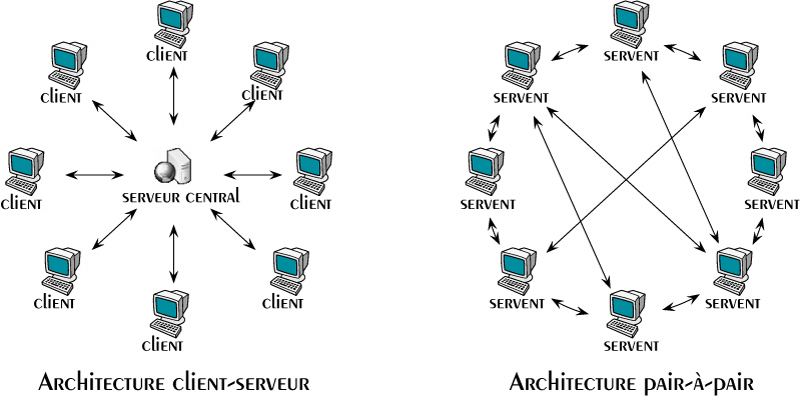
\includegraphics[width=15cm,height=8cm]{../Images/p2p-85145.png}\\
	\caption{Schéma des architectures pair à pair et client/serveur}
	\label{P2P/ClServ}
	\end{figure}


\newpage
\section{Mécanismes d'amélioration existants}
	\subsection{Area Of Interest}
	Dans plusieurs articles, la notion de \textit{Area Of Interest}~\cite{1403002,1267692,1015507} va apparaître ce qui montre l'utilité de ce mécanisme. Nous pouvons déjà retrouver ce principe sous le nom de \textit{Local Awareness} dans Sollipsis, l'idée principale de ce mécanisme est qu'une entité n'a pas besoin de connaître l'ensemble du monde virtuel à chaque instant. Alors nous allons mettre en place une zone dans laquelle l'entité sera tenue informée des différentes modifications qui seront faites sur les objets et les autres entités qui se trouvent dans la zone (voir schéma~\ref{AOI}). Si une entité modifie sa représentation virtuelle, seulement les entités qui sont dans sa zone seront directement informées.\\

	%\subsubsection{Mercury}
	\par Dans Mercury~\cite{1015507}, le concept d'Area Of Interest va pouvoir être utile avec le mécanisme de publish-subscribe qui est mis en place. Ce mécanisme de publish-subscribe permet l'abonnement et le désabonnement aux mises à jour d'un objet, et il permet donc d'envoyer un objet vers les nœuds qui sont abonnés.\\
	%\subsubsection{Colyseus}
	\par Colyseus~\cite{1267692} est un travail postérieur à Mercury, les principes sont les mêmes avec l'utilisation de \textit{range-queriable} DHT ou de DHTs pour stocker les informations. Les \textit{range-queriable} DHTs vont s'organiser en un overlay circulaire où chaque nœud adjacent est responsable d'une suite continue de clés. Grâce à cela, il sera possible de prendre les coordonnées "x" comme clé et ainsi les performances seront bien meilleures qu'avec des DHTs normales (aléatoire). Les différents résultats réalisés montrent bien que les \textit{range-queriable} DHTs utilisent moins de bande passante que les DHTs normales. \\
	%\subsubsection{Donnybrook}
	\par Dans Donnybrook~\cite{1403002}, le concept d'Area Of Interest fait référence au travail réalisé dans Colyseus. Comme chaque joueur envoie ses mises à jour à chaque joueur qui se trouve dans sa zone, il faut une limitation du nombre de joueurs dans une même zone. Donnybrook introduit la notion de \textit{player's interest set}, un joueur va pouvoir se concentrer sur un nombre fixe de joueur (cinq dans l'article), à la différence du nombre d'objet dans l'AOI qui peut varier. Un mécanisme d'abonnement sera mis en place pour s'échanger les informations entre les joueurs. Un mécanisme d'\textit{intérêt estimé} est mis en place pour définir les joueurs qui feront partis de son \textit{interest set}. Plusieurs critères sont pris en compte pour choisir les joueurs qui seront sélectionnés. Trois principales propriétés sont prises en compte: la proximité spatiale entre les joueurs, les objectifs des joueurs et les interactions récentes que les joueurs peuvent avoir eu entre les deux joueurs.\\
	\vspace{5mm}
        \begin{figure}[!h]
        \centering
        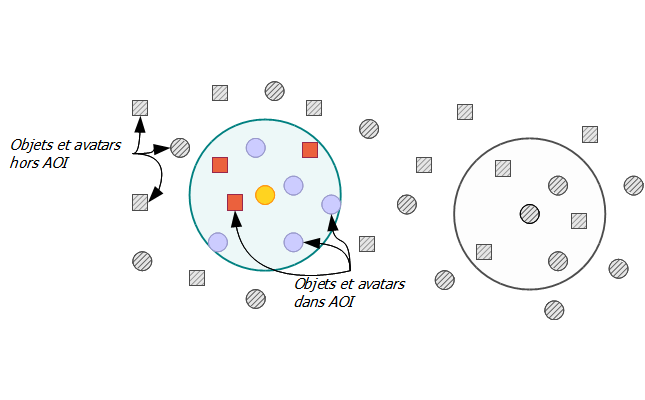
\includegraphics[scale=0.65]{../Images/AOI.png}\\
        \caption{Principe de l'\textit{Area Of Interest}}
        \label{AOI}
        \end{figure}
	\vspace{5mm}
	\subsection{Découpage de la carte}
	Pour plusieurs raisons, dont la tenue en charge, le monde a été découpé en plusieurs zones. Différentes techniques pour le découpage ont été étudiées, l'une des plus courantes est d'utiliser le découpage grâce au découpage de Voronoi~\cite{1016552}, c'est de cette technique que la triangulation de Delaunay s'inspire. Les découpages suivant ces principes sont répandus car un découpage aléatoire ne prendrait pas en compte la densité des objets dans le monde qui peut être très variable entre les régions. Le principe est de découper la monde en zone en fonction de la distance entre les différents objets qui se trouvent dans l'environnement. Dans une région, on aura un objet qui sera entouré de ses voisins. La frontière entre la région de deux voisins se trouve au milieu d'une droite séparant les deux voisins. Comme il est possible de voir sur le schéma~\ref{Voronoi}, les zones ont des formes et des tailles qui sont différentes. Nous avons ainsi des zones qui comprennent un seul nœud. La différence entre la triangulation de Delaunay et le découpage de Voronoi est que pour la première, les arrêtes seront les droite entre les sommets si ils sont voisins et dans le deuxième cas, les arrêtes seront formés grâce aux médiatrices des arrêtes de la triangulation de Delaunay.\\ 
	\vspace{5mm}
        \begin{figure}[!h]
        \centering
        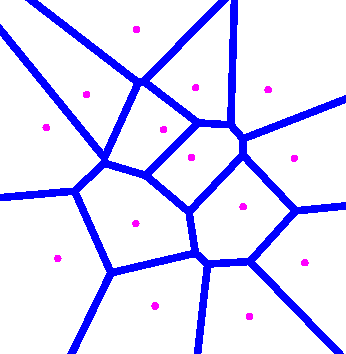
\includegraphics[scale=0.45]{../Images/voronoi.png}\\
        \caption{Principe du découpage de Voronoi}
        \label{Voronoi}
        \end{figure}
        \vspace{5mm}

	\subsection{Overlays}
	Plusieurs travaux sur la modification de l'overlay ont été fait~\cite{999375,10.1109/SRDS.2006.33,citeulike:6040284}, le but principal de ces travaux est de mettre en place un overlay qui puisse facilement s'adapter aux besoins des nœuds.
		\subsubsection{Semantic overlay}
			Le but principal de cet overlay sémantique~\cite{999375} est de créer des liens entre des nœuds qui s'intéressent aux mêmes documents, car la recherche de fichiers est devenu très importante au moment de l'arrivée des logiciels de partage de fichiers tel que Napster, Gnutella, KaZaA, etc. L'approche consiste à constituer des groupes sémantiques avec les documents et de construire un overlay au dessus du réseau pour chaque groupe. Le problème est donc d'identifier et de constituer des groupes efficacement. Trois stratégies ont été mises en place:
		\begin{itemize}
		\renewcommand{\labelitemi}{$\bullet$}
                	\item \textit{LRU:} Stratégie basé sur les éléments les plus récemment utilisés
                	\item \textit{History:} On maintient les liens sémantiques vers la même classe de préférence, cette technique oblige le maintien d'un nœud \textit{counter}.C'est une technique lourde en nombre de messages et en stockage, de plus il peut y avoir des problèmes avec les \textit{counters}.
	                \item \textit{Popularity:} Création de liens entre les nœuds du même type, introduction de deux paramètres: Numrep (nombre de réponse positive pour obtenir le document) et Lastreply (date de la dernière réponse )
        	\end{itemize}
	        Les résultats montrent que Popularity est l'algorithme le plus adapté, cette stratégie a un bon compromis entre efficacité et complexité de mise en place.

		\subsubsection{Application-Malleable Overlay}
			Il y a deux types d'overlay (structuré et non structuré), mais ces deux types ont un désavantage commun, ils ne sont pas flexibles. MOve~\cite{10.1109/SRDS.2006.33} souhaite mettre en place un overlay malléable, c'est à dire que les communications de l'application distribué vont influencer la structure de l'overlay. Les deux buts principaux sont d'optimiser les performances de l'overlay et de garder les propriétés de tolérance aux fautes et de passage à l'échelle. Les auteurs mettent en place deux types de liens:
		\begin{itemize}
	        \renewcommand{\labelitemi}{$\bullet$}
	                \item \textit{Lien non-applicatif:} Ils maintiennent l'overlay global proche d'un graphe aléatoire avec un faible degré de clustering (regroupement).
        	        \item \textit{Lien applicatif:} Ils  permettent de créer un graphe fortement connecté, pour regrouper les nœuds. Chaque nœud d'un groupe crée aléatoirement des liens applicatifs vers des membres du groupe. Cela va permettre une rapide propagation des états lors des updates et des messages applicatifs multicast.
        	\end{itemize}
        Cette solution offre différentes possibilités d'ajout de nœud, de détection de défaillance, de remplacement de lien, etc. \textit{group}-based applications influencent l'overlay sous-jacent en remplaçant les liens inter nodes par des liens entres les applications. L'algorithme maintient une bonne connectivité.
		\subsubsection{Voronoi-based Overlay Network}
		 	VON veut exploiter la localité des intérêts des utilisateurs pour maintenir la topologie pair à pair avec un faible \textit{overhead}. VON utilise un principe d'AOI dynamique, il utilise le découpage de Voronoi et chaque nœud est représenté par un site dans le diagramme. VON introduit trois procédures principales :
		\begin{itemize}
	        \renewcommand{\labelitemi}{$\bullet$}
                	\item \textit{Join Procedure:} Le textit{joining node} contacte le server pour avoir un ID unique, puis envoie une requête avec ses coordonnées à tous les nœuds existants. Création de la liste des voisins, mis à jour chez les voisins, etc.
                	\item \textit{Move Procedure:} Lorsque un nœud bouge ses coordonnées sont mises à jour chez ses voisins (gestion si nœud est à la limite de la région, si il y a des nouveaux voisins, etc).
                	\item \textit{Leave Procedure:} Le nœud se déconnecte (qu'importe sa raison et la manière) et ses voisins vont se mettre à jour.
        	\end{itemize}
        	VON permet de gérer un grand nombre d'utilisateurs et de garder un topologie consistante. Il y a beaucoup de messages introduits par l'AOI et si la vitesse des utilisateurs est trop importante, on a des problèmes pour notifier les nouveaux voisins.

		

	


\newpage
\section{Un système P2P pour MMOG: Solipsis}
	\label{solipsis}
	Solipsis est le ``socle'' du travail Blue Banana~\cite{keller-solipsis}, il est donc nécessaire de présenter les points importants pour la compréhension du travail Blue Banana. Solipsis introduit des propriétés qu'il va être important de comprendre et qui serviront lors de l'analyse des résultats des solutions implémentées durant le stage.
	\subsection{Introduction sur Solipsis} 
	\par Pour commencer, le fonctionnement global et les fonctionnalités importantes de Solipsis vont être présentés. Solipsis est fait pour accepter un nombre illimité d'utilisateurs et pour maintenir une cohérence suffisante pour un bon fonctionnement du système. Il peut être accessible par n'importe quel ordinateur, il peut fonctionner sur des ordinateurs peu puissants et avec des connections internet faibles (56Kbs) ou sans fil. Une fois les nœuds connectés, ils peuvent échanger des données telles que de la vidéo, du son, le mouvement d'avatar ou toutes choses affectant la représentation du monde virtuel. \\
	\subsection{Propriétés de Solipsis}
	Le monde de Solipsis est un tore à deux dimensions, chaque entité détermine sa position dans le monde et elle est responsable de cette dernière. Chaque utilisateur collecte les informations lui permettant de reconstituer son environnement virtuel local. Les connections entre les nœuds sont bidirectionnelles. 
		\subsubsection{Propriétés}
	Solipsis doit permettre aux utilisateurs de se déplacer à travers le monde, il faut pour cela que les deux propriétés locales suivantes soient respectées.
	\begin{itemize}
	\renewcommand{\labelitemi}{$\bullet$}
		\item \textit{Local Awareness:}\\
		Une entité doit être connectée avec tous ses plus proches voisins. Il est important de noter qu'une entité a la possibilité de connaître des entités en dehors de son environnement virtuel local. En revanche, cette propriété impose qu'une entité située à l'intérieur fasse partie des voisins de l'entité.	
		\item \textit{Global Connectivity:}\\
		Toute entité virtuelle doit se trouver à l'intérieur de l'enveloppe convexe contenant l'ensemble de ses voisins logiques. L'enveloppe convexe des entités est le plus petit polygone convexe formé par cet ensemble. Un mécanisme pour éviter qu'une partie du graphe soit isolée a aussi été mis en place.\\

		%Une entité doit connaître toutes les entités se trouvant dans son "champs de vision". Elle doit pouvoir détecter l'arrivée ou le départ d'une entité de son "champs de vision". Cette propriété est basée sur la Géométrie Informatique, elle assure qu'une entité ne "tourne pas le dos" à une partie du monde. L'enveloppe convexe des entités est le plus petit polygone convexe formé par cet ensemble. Un mécanisme pour éviter qu'une partie du graphe soit isolée a aussi été mis en place.\\
	\end{itemize}
        \vspace{1cm}
	\begin{figure}[!h]
	\centering
        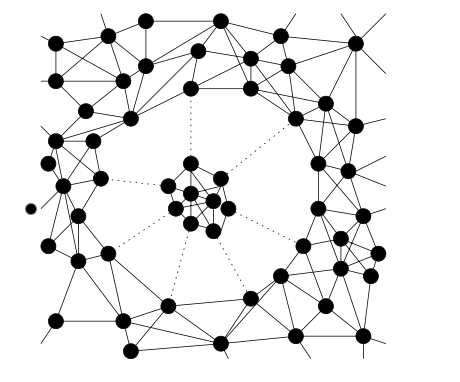
\includegraphics[scale=0.9]{./Ressources/Images/composant_isole1.png}\\
        \caption{Un composant connexe isolé et les connexions qui évitent la création d'une île}
        \label{Envelop_Convex}
        \end{figure}

		\subsubsection{Maintien des propriétés}
Solipsis a aussi des mécanismes de collaboration pour maintenir les propriétés précédentes, nous allons voir ces deux propriétés:
	\begin{itemize}
	\renewcommand{\labelitemi}{$\bullet$}
		\item \textit{Spontaneous Collaboration for Local Awareness:}\\
		 Pour vérifier la propriété \textit{Local Awareness}, il faut qu'une entité puisse connaître tous ses voisins à chaque instant. Pour faciliter cette connaissance du voisinage, et comme il y a un grand nombre de mouvements dans le monde virtuel, un système de collaboration entre les nœuds a été mis en place. Une entité pourra alors demander régulièrement à ses voisins s'ils détectent une nouvelle entité mais cela implique un grand nombre de messages inutiles et une perte temporelle de consistence. Pour éviter ces problèmes, une entité \textit{a} va prévenir une entité \textit{b} si une entité \textit{c} est en train de se diriger vers la zone de l'entité \textit{b}.
		\item \textit{Recursive Query-Response for Global Connectivity:}\\
		Il faut prévoir un mécanisme pour le maintien d'une entité dans l'enveloppe convexe. Quand une entité \textit{e} détecte deux entités consécutives, elle se lance immédiatement à la recherche d'une ou plusieurs entités dans la même zone en envoyant des messages dans la zone. \\ 
	\end{itemize}
        \vspace{1cm}
        \begin{figure}[!h]
	\centering
        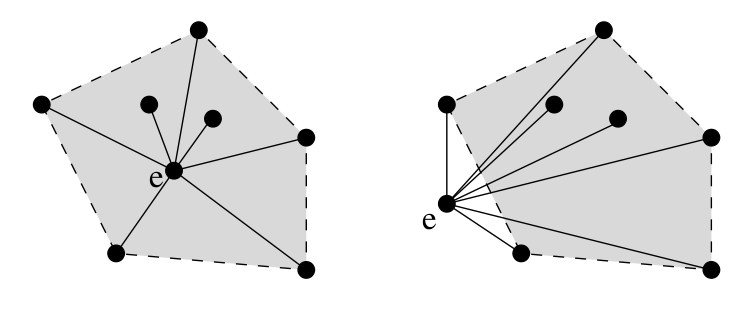
\includegraphics[scale=0.9]{./Ressources/Images/envelop_convex1.png}\\
        \caption{Deux différentes enveloppes convexes des voisins de \textit{e}. A gauche, \textit{e} respecte la règle de \textit{Global Connectivity} et à droite non.}
        \label{Envelop_Convex}
        \end{figure}


\newpage
\newpage
\section{Traces des utilisateurs dans les MMOGs}
	\label{trace}
 	Après avoir exposées des solutions qui ne prennent pas en compte la mobilité des joueurs, nous allons étudier celle-ci pour introduire la solution proposé par le travail Blue Banana. Pour étudier la mobilité dans les MMOGs, différentes techniques de collecte de traces ont été mises en place, nous présenterons celles-ci et expliquerons pourquoi ce travail de collecte est important pour améliorer les performances des solutions pair à pair pour les MMOGs.
	\subsection{Les différentes techniques de récupération de trace}
		\subsubsection{Les objectifs et les techniques de collecte de trace}
		\par Dans la littérature, il y a plusieurs études des traces d'utilisateurs de différents environnements virtuels~\cite{1326262,0295-5075-88-4-48007}. La plupart vont récupérer les traces des avatars sur des jeux vidéos tel que World Of Warcraft~\cite{wow} et Second Life~\cite{sl}. Ces études expliquent qu'il peut y avoir des différences entre des MMOGs. Par exemple dans Second Life l'environnement est beaucoup plus interactif (possibilités plus étendues de modification de l'environnement) que dans World Of Warcraft, ce qui peut affecter des différences de résultats des solutions en fonction du jeu~\cite{DBLP:journals/corr/abs-0807-2328,1613041}. \\
\par Ces travaux permettent de bien comprendre les différents comportements des joueurs, ils permettent ainsi de détecter les différents comportements en fonction des zones plus ou moins peuplées. Grâce à ces travaux, il est possible de faire ressortir des modèles montrant le comportement des avatars dans le monde virtuel. Ces modèles permettent de mettre en place une distribution spatiale des avatars, qui sera plus cohérente que dans les recherches où les distributions étaient uniformes~\cite{Knutsson04peer-to-peersupport}. Différentes mesures vont apparaître comme: le nombre de joueurs, le nombre d'arrivées et de départs, le temps moyen d'une session, la distribution des joueurs, etc. L'étude des traces des joueurs permet aussi de détecter les tricheurs qui utilisent souvent des bots~\cite{0295-5075-88-4-48007}. \\
		%\subsubsection{Les techniques de collecte des traces}
	\par Certaines techniques utilisent un bot qui est introduit dans le jeu et qui va récupérer des informations sur les autres joueurs. Le bot va rapatrier des informations à intervalles réguliers, il sera alors possible d'analyser les déplacements et vérifier les modèles. Une librairie open source \textit{libsecondlife} a été développée pour collecter les traces des joueurs de Second Life, à l'aide d'un bot~\cite{DBLP:journals/corr/abs-0807-2328}. Pour vérifier que les données récupérées sont cohérentes, une technique de positionnement de sept bots dans une région a été mise en place. Quatre bots statiques sont placés à chaque coin de la région, un autre statique va se placer au centre et deux autres vont bouger suivant un schéma défini. Il est alors possible d'enregistrer les positions des avatars se trouvant dans la région et les enregistrements des informations seront réalisés sept fois (par chaque bot). Une comparaison des données des sept bots est alors effectuée pour voir si des déviations existent entre les valeurs et si elles sont importantes.\\  
 		\subsubsection{Limitations de la collecte des traces}
	Des limitations existent pour la collecte des traces. Une des premières est que les mondes virtuels sont très souvent découpés en région ou en île, or les bots que nous introduisons ne peuvent pas traverser les régions et ils ne peuvent pas, par exemple, suivre des avatars. Dans~\cite{DBLP:journals/corr/abs-0807-2328}, la possibilité de différencier un avatar qui va dans une autre région et un qui quitte le jeu n'est pas possible. Il n'est pas possible de savoir ce que va faire l'avatar en dehors de la zone. Il y aussi un problème avec la détection des avatars qui se trouvent sur des objets et il n'y pas de prise en compte de la coordonnée \textit{z}. Une autre limitation de la collecte des traces est qu'elle se fait en très grande majorité de façon manuelle, il est donc très long et fastidieux de récupérer un nombre de traces suffisant pour effectuer des bonnes analyses. La collecte de trace peut aussi avoir des problèmes de passage à l'échelle car les systèmes de collecte existants travaillent à une petite échelle. Par exemple dans Second Life, le monde étant découpé en îles indépendantes, l'addition des traces collectées sur chaque île pour en faire une étude globale, n'est pas cohérente.

	\subsection{Observations des traces}
	 Beaucoup d'observations sur les déplacements des avatars dans les mondes virtuels ont pu être réalisé grâce à la collecte de toutes ces traces. La collecte des traces a aussi permis de faire valider ou invalider des modèles qui avaient été mis en place sans étude des traces~\cite{DBLP:journals/corr/abs-0807-2328}. 
		\subsubsection{Hotspots}
	Une des observations qui est ressortie de ces études est l'existence de différentes zones dans le monde. Une autre observation est que les mouvements des avatars sont très différents en fonction de la zone où ils se trouvent. Deux types de zones peuvent se dégager: des zones très peuplées avec des avatars ayant des mouvements très aléatoires et lents (Hotspots), et des zones qui sont entre les zones peuplées, où les avatars se déplacent rapidement et suivent souvent une trajectoire rectiligne (Waypoints). Des phénomènes de déplacement en groupe ont aussi pu être repérés~\cite{15141312}. \\
		\subsubsection{Waypoints}
	Comme nous pouvons le voir dans le schéma~\ref{sch_trace}, il y a des "routes" entre les différents points de regroupement. Ces routes vont nous permettre de mieux anticiper les déplacements des avatars entre les \textit{Hotspots}.
        \vspace{1mm}
        \begin{figure}[!h]
        \centering
        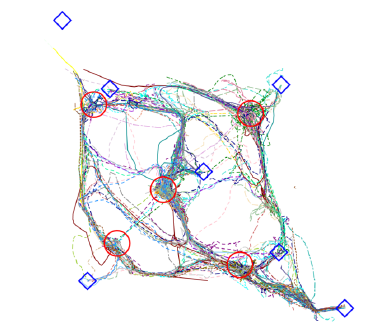
\includegraphics[scale=0.75]{./Ressources/Images/trace.png}\\
        \caption{Battle 980 movement paths}
        \label{sch_trace}
        \end{figure}	
        \vspace{1mm}
\newline
	L'étude des traces a aussi permis de détecter les habitudes des joueurs, comme le fait qu'ils jouent à certaines heures plutôt que d'autres et avec des durées de connexion différentes en fonction de l'heure de la journée.


\newpage
\section{Prise en compte de la mobilité: Blue Banana}
	\label{BlueBanana}
	Il nous a été possible de voir, dans les chapitres précédents, des mécanismes qui permettent de faire évoluer le système en réaction à des événements. Solipsis ne pourrait difficilement fonctionner dans un monde avec des traces réalistes. En prenant en compte les études des traces des joueurs, Blue Banana a permis de mettre en place un mécanisme d'anticipation des mouvements des avatars pour mieux s'adapter.
	\par Blue Banana présente une solution aux différents problèmes que peut rencontrer une architecture pair à pair dans les MMOGs. La mobilité des avatars implique de nombreux échanges de données à travers le réseau pair à pair. Comme les overlays de l'état de l'art n'anticipent pas cette mobilité, les données nécessaires ne seront pas chargées à temps, ce qui conduit à des défaillances transitoires au niveau applicatif. Blue Banana a été réalisée pour résoudre ce problème, il modélise et prédit les mouvements des avatars ce qui permet à l'overlay de s'adapter par anticipation aux besoins du jeux.
	\subsection{Solutions introduites}
	Blue Banana est implémenté au dessus de Solipsis qu'il a été possible d'étudier dans le chapitre~\ref{solipsis}. Plusieurs observations ont été faites et différentes optimisations en sont ressorties. Il nous a été possible d'observer plusieurs types de zone (dense ou non, cf.~\ref{trace}) et que les mécanismes d'adaptation sont trop tardifs pour être mis en place dans la réalité (le chargement des données sera trop lent).
	\subsubsection{Les états de l'avatar}
	\label{Automate}
	Une des premières innovations qui a été introduite est la distinction de plusieurs états d'un avatar. Comme il a été possible de voir dans le chapitre sur la collecte de traces, un avatar se comporte différemment en fonction des zones du monde. Trois états ont donc été introduits:
	\begin{itemize}
	\renewcommand{\labelitemi}{$\bullet$}
		\item \textbf{H}(alted): l'avatar est immobile.
		\item \textbf{T}(ravelling): l'avatar se déplace rapidement sur la carte et il a une trajectoire droite.  
		\item \textbf{E}(xploring): l'avatar est en train d'explorer une zone, sa trajectoire est confuse et sa vitesse est lente.
	\end{itemize} 
	Le changement d'état de l'avatar se fait en fonction de la vitesse de celui-ci, si la vitesse devient supérieure à une borne définie et que l'avatar est dans l'état E alors l'avatar passe en état T. Ce modèle pourrait être affiné par la suite en prenant en compte l'accélération ou l'historique des mouvements. Sur la figure~\ref{automateMob}, nous pouvons mieux distinguer les différents changements d'état. Chaque nœud va agir en fonction de cette automate, il sera initialisé à l'état \textbf{H}(alted). \\
	

	\begin{figure}[!h]
        \centering
        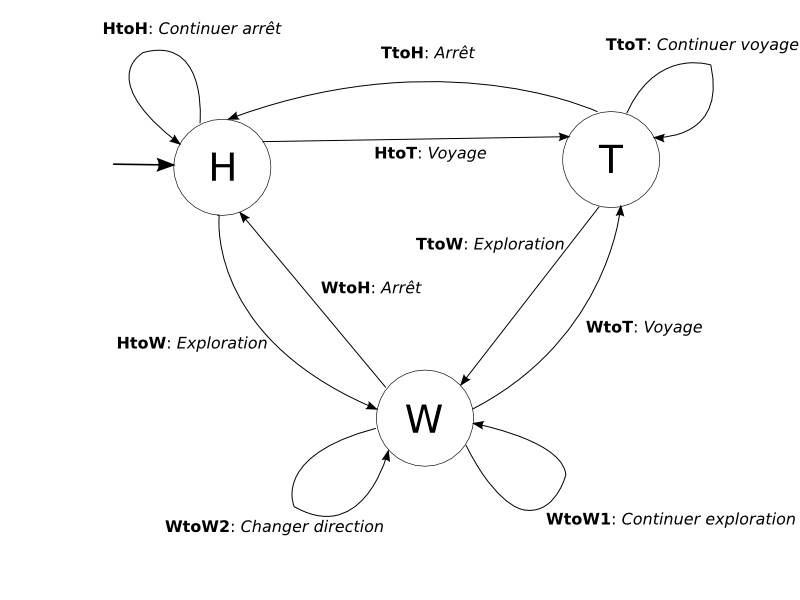
\includegraphics[scale=0.4]{./Ressources/Images/automate.png}
        \caption{\textit{\small Automate décrivant les mouvements d'un avatar. \textbf{En gras}: le nom de la transition, en \textit{italique} sa sémantique}}
        \label{automateMob}
        \end{figure}




	\subsubsection{Anticipation des mouvements}
	Un autre mécanisme a été mis en place, il s'agit d'anticiper les mouvements d'un avatar, pour cela deux suppositions sont faites: seulement une prédiction courte est cohérente, et plus l'avatar se déplace rapidement, plus il y a de chance qu'il continue dans la même direction~\cite{191}. Comme nous pouvons voir sur la figure~\ref{Propa_Algo}, en fonction du vecteur de mouvement de l'avatar, le nœud B, s'il est dans l'état \textbf{T}, va chercher des nœuds qui se trouvent sur la trajectoire probable de l'avatar, tant que son ensemble de voisins n'est pas plein. Le nœud B va envoyer un message aux voisins qui sont le plus près de lui par rapport au vecteur de mouvement. Un mécanisme pour évaluer si le nœud n'est pas trop près, et donc rapatrier des données ne servirait pas car le temps des communications serait supérieur au temps du déplacement de l'avatar. Un des risques est de rapatrier des nœuds qui seront inutiles si l'avatar va changer de direction ou d'état. L'amélioration de ce point fait parti des futures pistes pour améliorer l'algorithme d'anticipation des mouvements.\\
	\vspace{5mm}
        \begin{figure}[!h]
        \centering
        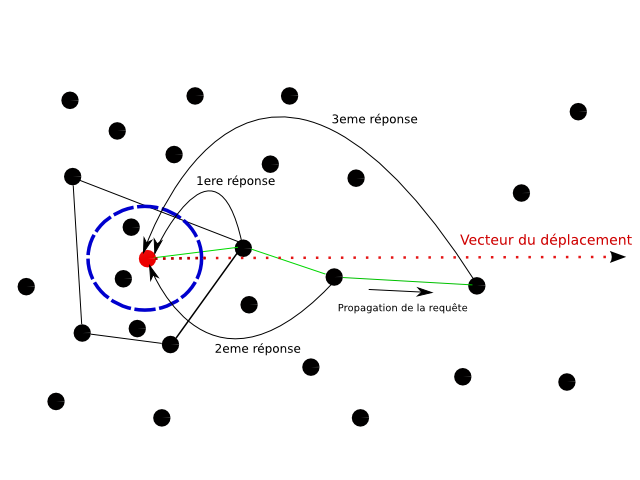
\includegraphics[scale=0.5]{./Ressources/Images/propagation_algo.png}\\
        \caption{Algorithme de propagation}
        \label{Propa_Algo}
        \end{figure}
        \vspace{5mm}
	\subsection{Expérimentations et Résultats}
		Le travail a été testé sur le simulateur à évènements discrets PeerSim ~\cite{peersim}, les expérimentations ont eu pour objectif de comparer Solipsis avec et sans Blue Banana.
		\subsubsection{Le simulateur PeerSim et la description des expérimentations}
		\par PeerSim est un simulateur de réseau pair à pair, qui a deux modes de fonctionnement: par cycles ou par évènements. C'est une API riche et modulaire qui est codée en Java, c'est une composante du projet BISON de l'université de Bologne (Italie). Ce simulateur permet de simuler un large nombre de machines et de tester différentes configurations du réseau. Le simulateur va faire des simplifications sur les couches réseau et les contraintes physiques (latence, pannes, ...). Chaque nœud est considéré comme un module qui va échanger des messages avec les autres nœuds du système. La plupart des plateformes de simulation est basée sur le modèle à évènements discrets. Il est possible de distinguer deux entités: les nœuds et les messages. Le temps va seulement évoluer à chaque nouvel évènement sur un nœud.
		%\subsubsection{Description des expérimentations}
		\par Au départ de la simulation, une carte initiale des traces est introduite dans le simulateur, la carte provient d'une étude de La et Michiardi~\cite{LM-wosn08} dans Second Life. Ensuite, le simulateur va initialiser l'overlay de Solipsis et vérifier que les deux règles de Solipsis sont bien respectées sur chaque nœud, nous insérerons ensuite le reste des traces. Il faut aussi régler les différents paramètres du simulateur (nombre d'avatar, surface du monde, densité, accélération des avatars, vitesse de connection, etc). Plusieurs métriques sont mises en place pour évaluer les résultats:
	\begin{itemize}
	\renewcommand{\labelitemi}{$\bullet$}
		\item \textit{Violation of Solipsis fundamental rules}: Regarde si les propriétés de \textit{Global Connectivity} et de \textit{Local Awareness} sont respectées.
		\item \textit{Knowledge of nodes ahead of the movement}: Mesure pour les avatars qui se déplacent rapidement, le temps moyen pour qu'il connaisse un nœud qui sera sur sa trajectoire.
		\item \textit{Exchanged messages count}: Mesure l'impact de Blue Banana sur le réseau, cela va compter le nombre de messages introduits par Blue Banana et Solipsis.
	\end{itemize}
		\subsubsection{Les résultats}
		Les résultats les plus intéressants montrent que Blue Banana diminue les transitions en échec de 55\% à 20\%, augmentent la connaissance des prochains nœuds de 270\% et cela en créant un overhead de seulement 2\%. Les résultats montrent que le mécanisme d'anticipation introduit par Blue Banana aide l'overlay de Solipsis à s'adapter à temps et à réduire significativement le nombre de violation des règles de Solipsis (de 55\% ou 80\% à 20\%). 


\newpage
\section{Introduction des Solutions}
\label{introSolutions}
	Le problème a résoudre, durant le stage, est d'améliorer la réactivité des réseaux pair à pair pour les MMOGs. La réactivité des protocoles pair à pair existants ne permet d'assurer la latence suffisante pour les application vidéoludique multijoueur. Blue Banana permet l'amélioration de la réactivité en rapatriant des données qui nous seront nécessaires dans un futur proche. Le travail effectué dans Blue Banana (cf \ref{BlueBanana}, page \pageref{BlueBanana}) s'intéresse à une partie du jeu bien définie, cette partie comprend les déplacements entre les zones denses. Durant le stage, il a donc fallu chercher des solutions qui permettraient d'améliorer le travail existant. Plusieurs pistes de solution ont été trouvées, deux de ces pistes ont été implémentées et testées. Les deux solutions implémentées, durant le stage, sont la mise en place d'un cache pour les zones denses de l'environnement, et la modification du rapatriement des données réalisé dans Blue Banana, pour les déplacements entre les zones denses.
\begin{table}[!h]
  \begin{center}
    \begin{tabular}{|c|c|}
      \hline
      Solution & Partie Améliorée \\
      \hline
      Introduction d'un cache  & Dans les zones denses \\
      Amélioration du préchargement & Entre les zones denses \\
      \hline
    \end{tabular}
  \end{center}
  \label{tab:config2}
  \caption{Tableau récapitulatif des solutions ajoutées durant le stage}
\end{table}
\par Dans la première solution, l'intérêt s'est porté sur une partie du jeu qui n'était pas étudiée dans Blue Banana. Le comportement des avatars dans les zones denses restait le même que dans Solipsis, nous avons donc décidé d'améliorer le fonctionnent dans ces zones denses. A l'intérieur de celles-ci, les joueurs se déplacent de façon désordonnée et bougent la plupart du temps dans un secteur restreint. L'utilisation d'un cache est alors apparu comme une solution d'amélioration. Le principe du cache est très simple, un nœud oubliait des voisins dont il pourrait avoir besoin dans un futur plus ou moins proche (en fonction de la mobilité dans le jeu), la mise en place du cache va permettre de garder un nombre \textit{N} de nœuds dans l'éventualité où le nœud revienne dans une zone où il est déjà venu (voir Schéma \ref{mouveDense}). Nous expliquerons les différentes solutions que nous avons testé pour le cache, et pourquoi celles que nous avons retenu fonctionnaient mieux.
        \begin{figure}[!h]
        \centering
        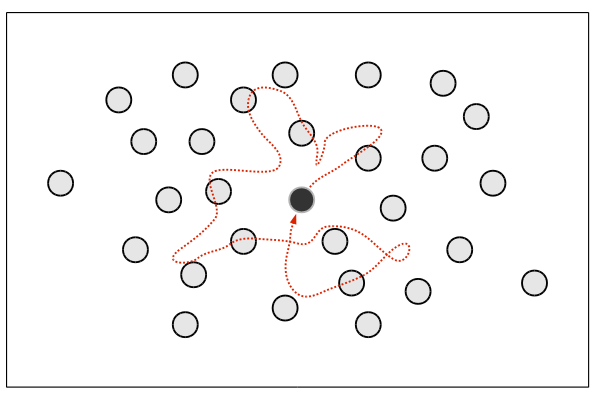
\includegraphics[scale=0.25]{./Ressources/Images/mouvementsZoneDense.png}\\
        \caption{Exemple d'une trajectoire d'un joueur dans une zone dense}
        \label{mouveDense}
        \end{figure}
\par La deuxième solution a consisté à modifier le préchargement des données réalisées dans Blue Banana, pour que celui-ci se fasse de manière plus fine. Les modifications que nous avons introduites doivent permettre d'économiser des messages et d'améliorer la cohérence de la topologie. Différentes techniques et algorithmes ont été testés, les plus importantes seront décrites et expliquées.
\par Les deux solutions mises en place permettent d'améliorer le travail qui avait déjà été effectué dans Blue Banana. Un des intérêts de nos solutions est qu'elles permettent d'améliorer une partie de l'environnement qui n'avait pas était traité (cache pour les zones denses), et d'améliorer un travail existant.




\newpage
\section{La mise en place d'un cache pour les zones peuplées}
\subsection{Introduction}
Comme nous avons pu le voir dans la partie~\ref{introSolutions}, la mise en place d'un cache pour les zones peuplées permettrait d'améliorer la réactivité dans l'état \textbf{W}(andering). L'avantage de cette solution était de s'intéresser à une partie qui n'avait pas encore été étudiée dans Blue Banana. Nous avons donc inséré un cache pour chaque nœud de l'environnement, celui-ci va fonctionner dans la continuité de liste des voisins d'un nœud. Nous expliquerons comment nous avons inséré le cache dans le code existant, les différentes stratégies que nous avons pu mettre en place et les différents paramètres qui vont influencer le fonctionnent du cache. Nous avons aussi permis l'utilisation du cache pour aider ses voisins quand ceux-ci cherchent des nœuds.
 
\subsection{Explications de la mise en place du cache}

\subsubsection{Le fonctionnement global et la mise en place du cache dans Blue Banana}
Le fonctionnement global du cache consiste à garder en mémoire un certain nombre de nœuds qui faisaient parti de la liste des voisins. Ainsi, comme les mouvements de l'avatar sont désordonnés, il est possible qu'il retourne vers des nœuds qu'il vient de quitter. 
\par Sur la figure~\ref{cacheW}, nous pouvons voir les principales étapes du fonctionnement du cache. Au départ le cache et la liste des voisins sont remplis de différents nœuds. A l'étape 2, le nœud courant (rouge) se déplace et trouve des nouveaux voisins, ceux-ci sont insérés à sa liste des voisins. Deux nœuds sont alors déplacés vers le cache, ce qui pousse deux nœuds hors du cache. A la dernière étape, le nœud courant revient vers une zone qu'il connait (nous détaillerons après le mécanisme de recherche dans le cache) et il trouve deux nœuds dans son cache qui pourraient lui servir pour reconstruire son voisinage. Deux nœuds du cache sont alors insérés dans la liste des voisins du nœud courant, ce qui envoie deux nœuds de cette liste vers le cache. Dans cette exemple, plusieurs nœuds peuvent se déplacer en même temps, ce qui est le cas dans une seule des solutions de cache mise en place.
	\begin{figure}[!h]
        \centering
        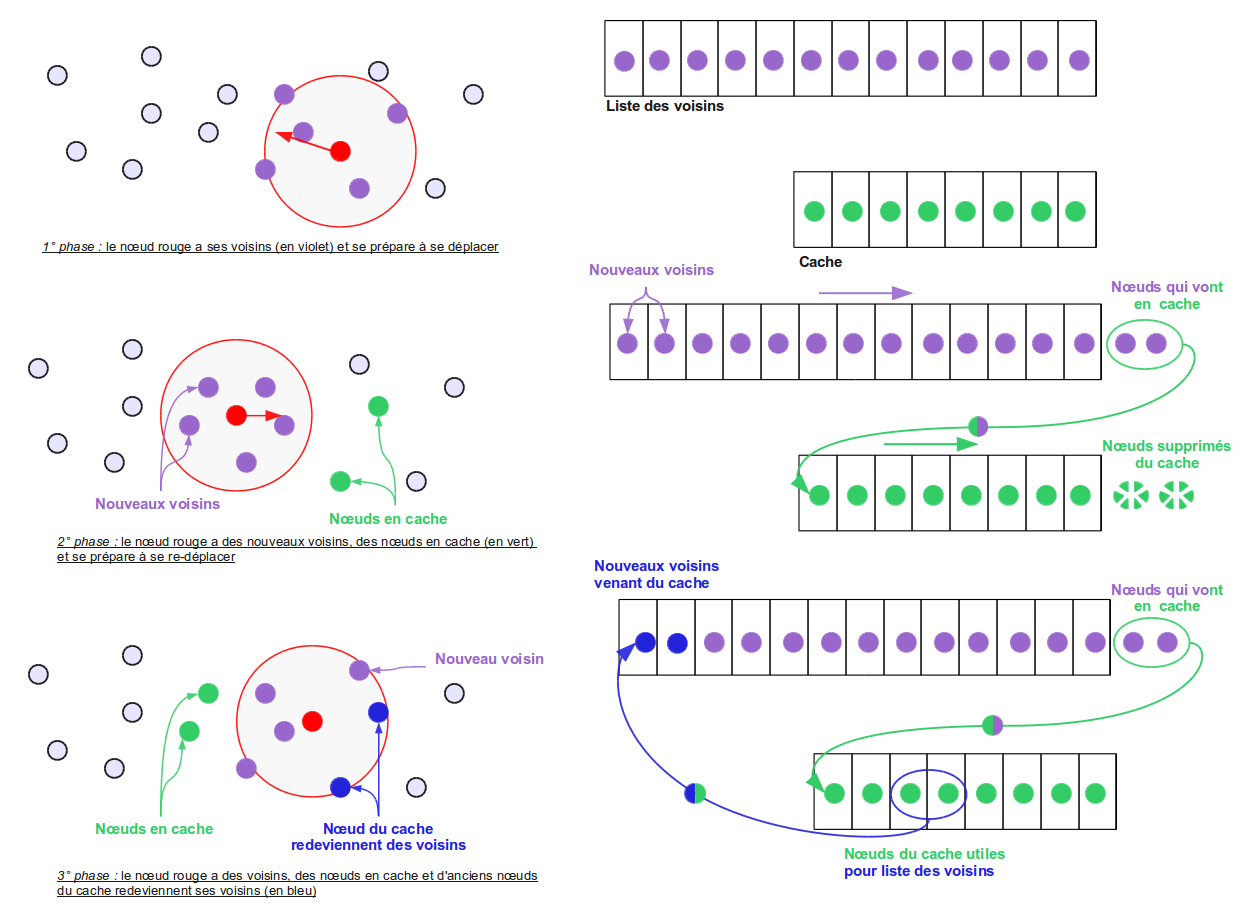
\includegraphics[scale=0.35]{./Ressources/Images/cacheWextends.png}
        \caption{Exemples du fonctionnement global du cache}
        \label{cacheW}
        \end{figure} 
\par Cette solution permet d'économiser des messages de découverte des voisins (SEARCH) dans le cas de changements de direction fréquents. Il doit aussi nous permettre d'économiser des messages de connexions et de déconnexion. Nous verrons dans la partie~\ref{resObsCache} les différents gains de la mise en place du cache, mais aussi les limites de celui-ci. Le cache est donc le prolongement de la liste des voisins pour nœud, mais contrairement à celui-ci , il n'est pas à jour, car un nœud est ajouté dans le cache avec les dernières informations qui étaient disponibles dans la liste des voisins. 
\par Nous avons donc mis en place un système de mise à jour du cache, pour avoir des informations les plus exactes possibles sur chaque nœud. Mais ce système coûte cher en nombre de messages, et cela est encore plus vrai plus le cache est grand. Un mécanisme de datation des éléments du cache permet de savoir depuis quand date les informations de chacun. Ce mécanisme nous permet de contacter un nœud pour savoir s'il se trouve toujours à peu près au même endroit, et ainsi l'ajouter ou non à notre voisinage. Ces paramètres sont en option et nous verrons dans la partie~\ref{resObsCache} quelles sont les meilleures combinaisons d'options et si elles sont toutes utiles ou non.

\subsubsection{Les différentes versions du cache}

Deux versions, pour le fonctionnent du cache, ont été testées durant la phase de codage. Nous parlons ici de la gestion des données dans le cache et non de la recherche dans celui-ci qui se fera juste après. Au départ le cache était géré selon le principe \textit{First In First Out}. La gestion du cache se faisait sans tenir des mises à jour de certaines données qui peuvent avoir lieu lors d'une requête en échec vers un nœud du cache. Les données du nœud ayant trop bougé sont alors rafraichies dans le cache. Une gestion du cache en fonction de la localité a aussi été mise en place, ce qui permet de faire sortir du cache les nœuds les plus éloignés de la position actuelle du nœud.
\par Deux implémentations ont aussi été testées pour la recherche dans le cache, l'une renvoie un résultat et l'autre renvoie plusieurs nœud à ajouter. Les tests montrent que la deuxième implémentation donne de meilleurs résultats (voir chapitre~\ref{resObsCache}).


\subsubsection{La modification du code existant pour insérer la recherche dans le cache}

 Avant de regarder les algorithmes de recherche dans le cache, nous allons expliquer comment ils sont appelés et quelles sont les modifications introduites par rapport au code original. Lorsqu'un nœud rentre dans la fonction \textit{solipsisRecoverTopology} si le nœud est dans l'état \textbf{W}(andering) alors on passe dans la fonction \textit{MaintainTopology}, sinon on effectue le traitement normal. Nous pouvons voir ci-dessous une partie du code de la fonction MaintainCache. Pour commencer, nous testons l'état de l'entité appelante, ensuite en fonction de la stratégie, nous faisons un traitement particulier. Nous nous concentrerons sur la stratégie de base qui ajoute un seul nœud. La fonction de recherche nous renvoie donc un résultat. S'il n'est pas nul et que sa date de mise à jour n'est pas trop ancienne, nous enlevons le nœud du cache, ajoutons le nœud à la liste des voisins et renvoyons 1 à la fonction appelante pour lui signifier que le traitement à été fait. Ensuite en fonction de la valeur de l'option \textit{contact\_node}, nous contactons ou non le nœud renvoyé par la fonction de recherche. Nous faisons ceci pour savoir s'il a beaucoup bougé depuis le dernier moment où nous l'avons vu. Nous retournons 0 pour signifier à la fonction appelante qu'aucun nœud n'a été ajouté et qu'elle peut faire le traitement de base.

\lstset{numbers=left,basicstyle=\scriptsize, numberstyle=\tiny, stepnumber=5, numbersep=5pt}

\lstinputlisting[title={Partie du code de la fonction MaintainCache},label={codeMaitainTopology}]{./Ressources/Documents/MaintainTopology.java}



\subsubsection{Les algorithmes de recherche dans le cache}
\par Nous allons expliquer de quelle façon les données sont recherchées dans le cache, et nous détaillerons les différentes pistes que nous avons testé. La méthode n°1 sélectionne les nœuds en terme de distance. L'idée est de récupérer les nœuds les plus proches de notre nouvelle position. Cette solution a était assez simple à mettre en place car il s'agit d'une simple comparaison de distance. 
\begin{table}[!h]
  \begin{center}
    \begin{tabular}{|c|c|c|c|}
      \hline
      N° & Critère de sélection & Avantages & Inconvénients\\
      \hline
      	1 & Comparaison distances & Simplicité & Distance~$\ne$~utile, aide pas enveloppe\\
      	2 & Aide enveloppe & + Enveloppe OK & - bon règles Solipsis\\
      	3 & Zone de connaissance & Simplicité & aide pas enveloppe\\
      \hline
    \end{tabular}
  \end{center}
  \label{tab:config1}
  \caption{Tableau montrant les valeurs utilisées pour la configuration n°1}
\end{table}


\par La méthode n°2 prend en compte la capacité d'un nœud à aider à refaire l'enveloppe connexe du nœud courant. Nous avons alors implémenté une solution qui rendait un résultat positif si un nœud dans le cache permettait de reconstruire l'enveloppe du nœud (voir schéma~\ref{schemaEnvelopCache}). Cette solution a même été agrémentée d'un test si le nœud faisait avancer positivement l'enveloppe connexe mais ne la reconstruisait pas immédiatement.

	\begin{figure}[!h]
        \centering
        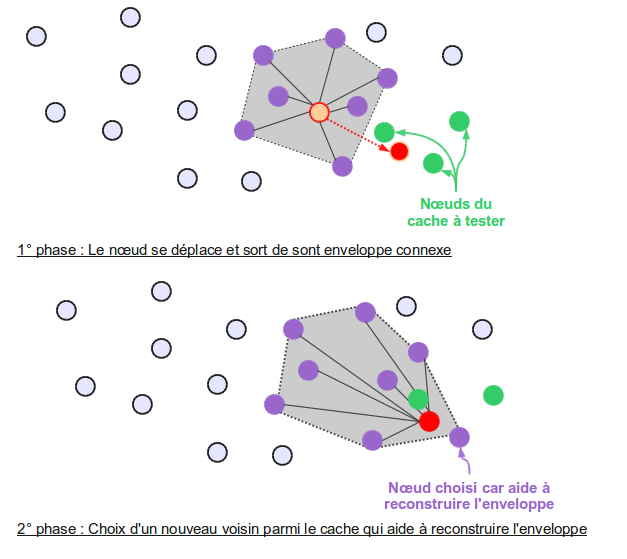
\includegraphics[scale=0.45]{./Ressources/Images/cacheReconstructEnvelop.png}
        \caption{Schéma montrant la solution de recherche dans le cache aidant à reconstruire l'enveloppe}
        \label{schemaEnvelopCache}
        \end{figure}
Le problème de cette solution est qu'elle privilégiait l'enveloppe connexe à la propriété de \textit{Local Awareness}. Car nous pouvons nous retrouver dans la situation, comme dans la figure~\ref{schemaEnvelopCache}, où un nœud ne fait pas parti de la liste des voisins alors qu'il se trouve dans l'enveloppe connexe. Cette solution nous donnait donc des résultats, pour les propriétés de Solipsis, qui pouvaient être moins bons que la version sans le cache.  

\par La dernière méthode, la n°3, celle qui est retenu dans l'implémentation, ressemble à la solution n°1. Chaque nœud comporte une zone de connaissance, nous avons donc décidé de nous servir de cette dernière pour réaliser les conditions dans la fonction de recherche. La fonction de recherche regarde si un nœud du cache est dans la zone de connaissance du nœud courant. Si plusieurs correspondent un système pour choisir aléatoirement est mis en place, comme dans la fonction de recherche de voisin original. Une autre fonction qui recherche en prenant en compte la région géométrique a aussi été mise en place, les résultats sont équivalents à la version avec la zone de connaissance.

\subsubsection{La mise en place de l'aide aux voisins grâce au cache}

Le cache d'un nœud va donc lui servir pour essayer de connaitre son environnement plus rapidement, mais il pourrait aussi aider les voisins du nœud. Dans cette optique, l'aide aux voisins a été mise en place. Ceci permet au cache d'avoir une autre utilisation, ce qui pourrait permettre d'économiser quelques autres messages. 
\par Lorsqu'un nœud cherche des voisins, il envoie un message SEARCH (voir schéma~\ref{schemaHelpCache}). Il suffit donc d'insérer une recherche dans le cache au bon endroit dans la fonction de traitement de ce message. Nous insérons donc, dans la fonction \textit{processSearchMsg}, une fonction de recherche dans le cache. Le nœud va tout d'abord regarder dans sa liste des voisins et si aucun ne correspond, nous regardons dans le cache si un nœud peut correspondre à la requête. La recherche dans le cache se fait, de façon similaire à une recherche dans le cache pour un nœud local, en utilisant la zone de connaissance que l'on aura préalablement transmis dans le message.

	\begin{figure}[!h]
        \centering
        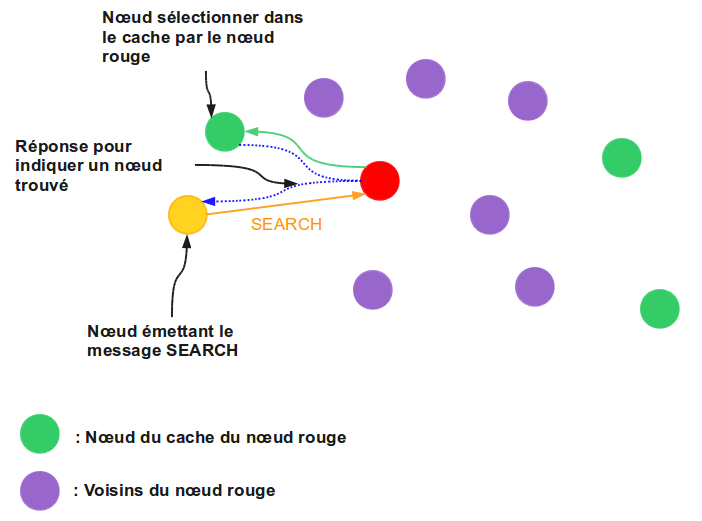
\includegraphics[scale=0.4]{./Ressources/Images/cacheHelp.png}
        \caption{Schéma montrant l'aide du cache pour le traitement d'un message SEARCH}
        \label{schemaHelpCache}
        \end{figure}

\subsection{Résultats et observations sur le cache}
\label{resObsCache}

Nous allons présenter les différents résultats sur le cache. Nous comparerons chaque version avec une version de base où l'on ne trouve ni cache ni prefetch, et avec une version avec le prefetch implémenté dans Blue Banana.
Les principales métriques pour comparer les différents résultats sont la cohérence de la topologie et le nombre de messages qui sont exprimés en fonction de la mobilité des avatars. Le calcul de la cohérence de la topologie consiste à mesurer, à chaque instant, le nombre de nœuds qui sont dans la zone de connaissance d'un autre nœud mais qui ne font pas parti des voisins de ce dernier.

\par Tout d'abord, nous allons regarder le nombre de cache Hit et Miss pour le cache normal. Il s'agit de voir le taux de réussite du cache et donc si ce mécanisme est souvent utlisé. Dans ces premiers résultats, le cache est configuré de tel sorte qu'il utilise l'aide aux voisins, mais qu'il ne contacte pas un nœud du cache s'il est trop vieux. Cette configuration ne va récupérer que les nœuds du cache qui sont très proches et qui ont été ajoutés au cache récemment (voir tableau ci dessous). La taille du cache correspond au nombre de nœud qu'il peut contenir, la limite de distance correspond à la distance à partir de laquelle nous ne récupèrerons pas le nœud. La limite de temps est la différence maximum qu'il doit y avoir entre le temps courant et la date de rafraichissement du nœud dans le cache (généralement l'ajout de celui-ci dans le cache). 
\begin{table}[!h]
  \begin{center}
    \begin{tabular}{|c|c|}
      \hline
      Paramètre & Valeur\\
      \hline
      Taille du cache & 25\\
      Limite de distance &  1500\\
      Limite de temps & 1500\\
      Contact Nœud & Faux\\
      Mise à jour du cache & Faux\\
      Aide aux voisins & Vrai\\
      \hline
    \end{tabular}
  \end{center}
  \label{tab:config1}
  \caption{Tableau montrant les valeurs utilisées pour la configuration n°1}
\end{table}


\par Nous pouvons voir que plus la mobilité augmente plus le nombre de cache Hit augmente et le nombre de cache Miss diminue (voir figure~\ref{courbesHitMiss:config1}). Cela est dû au fait que plus la mobilité augmente plus le cache aura des entrées récentes, car les nœuds vont changer de direction plus souvent et plus rapidement. Notre politique de cache ne prenant en compte que des nœuds récemment ajoutés au cache, les résultats en terme de cache Hit sont bien meilleurs. Nous pouvons aussi noter qu'il ya de moins en moins d'accès au cache car la somme des Hit et des Miss diminue, cela est du au fait que de plus en plus de nœuds sont dans un état \textbf{T}. 

	\begin{figure}[!h]
        \centering
        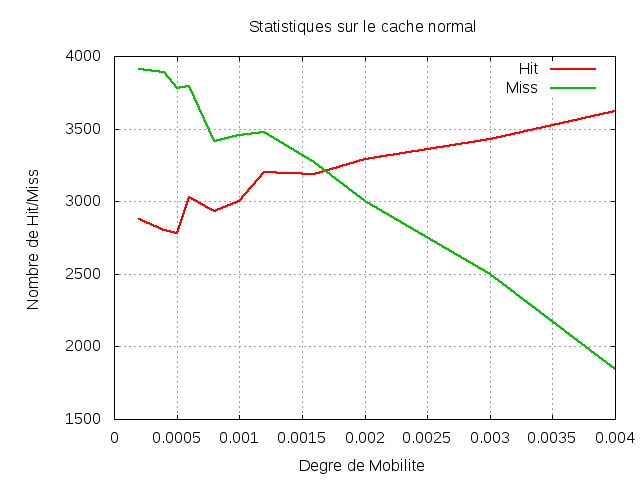
\includegraphics[scale=0.5]{../CacheCode/SolipsisPeersim/resultats/Courbes/Courbes_Final_Rapport/Cache_Stats_Normal.png}
        \caption{Schéma montrant les caches Hit et caches Miss pour le cache normal}
        \label{courbesHitMiss:config1}
        \end{figure}
\newpage
\par Ensuite nous pouvons observer le nombre de messages en fonction du degré de mobilité (voir figure~\ref{courbesNbMessCache:config1}). Les deux versions du cache vont nous permettre d'économiser des messages car lors d'un cache Hit nous ne faisons pas le traitement de base qui provoquait l'envoie d'un message. Le traitement du cache se fait sans coût en terme de message. Si l'on fait le traitement de base après le passage dans le cache, un gain en nombre de message sera tout de même réalisé. Ce gain résulte du fait que le nœud connaîtra mieux son environnement et la prochaine fois qu'il devra entrer dans la fonction \textit{MaintainCache} sera retardée. Ces observations sont les mêmes pour le cache à réponse simple et le cache à réponse multiple.  


	\begin{figure}[!h]
        \centering
        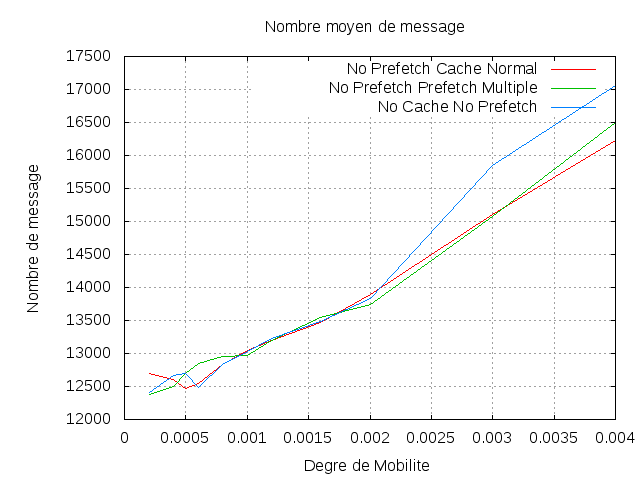
\includegraphics[scale=0.5]{../CacheCode/SolipsisPeersim/resultats/Courbes/Courbes_Final_Rapport/Nombre_Messages_Caches.png}
        \caption{Schéma montrant le nombre de messages}
        \label{courbesNbMessCache:config1}
        \end{figure}

Nous allons maintenant observer la cohérence de la topologie avec les différentes versions du cache. Les différences entre les versions avec cache simple et sans cache sont minime. Le nombre de cache Hit est pourtant en évolution avec la mobilité. Ces résultats peuvent s'expliquer du fait que si le cache trouve un nœud, la version sans le cache l'aurait peut être aussi fait mais avec l'envoie de messages. Il est possible que si nous augmentions les durées des communications, les résultats soient meilleurs. La fin du stage permettra de validé ou non cette possibilité.
\par La version du cache fonctionnant avec une recherche renvoyant plusieurs nœuds donne des résultats meilleurs que la version de base (sans cache et sans prefetch). Cette version donné aussi de meilleures résultats que la version avec un retour simple. Ce résultat est normal, car un plus grand nombre de nœud utile à la cohérence de la topologie et rajouté en un passage.

	\begin{figure}[!h]
        \centering
        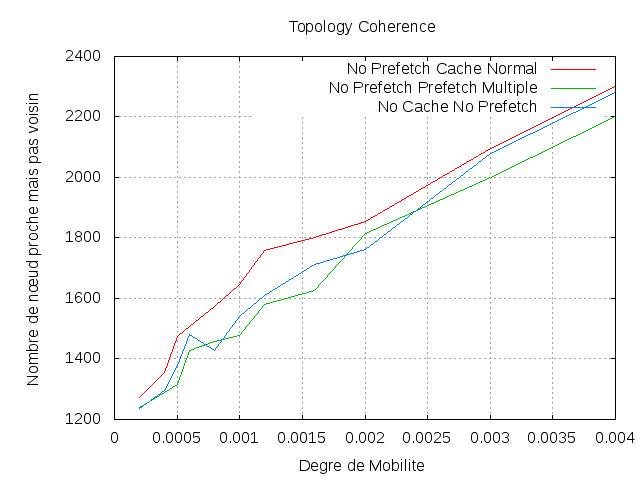
\includegraphics[scale=0.5]{../CacheCode/SolipsisPeersim/resultats/Courbes/Courbes_Final_Rapport/Topology_Coherence_Caches.png}
        \caption{Schéma montrant la cohérence de la topologie}
        \label{courbesTopoCohCache:config1}
        \end{figure}

\subsubsection{Résultats des autres implémentations}

Les mises à jour du cache permettent de récupérer toutes les nouvelles données correspondants aux nœuds stockés. Ces mises à jour permettent donc de moins se tromper entre les coordonnées stockées et les coordonnées effectives des nœuds. Mais cela ne veut pas dire que le cache va permettre de bien meilleur résultats. En effet, les nœuds mises à jour peuvent avoir beaucoup bougés et donc s'être éloignés du nœud courant. Les tests montrent une augmentation du nombre de messages qui est croissante avec le nombre de nœuds du cache et avec la fréquence du mécanisme de mise à jour. Une très légère amélioration de la cohérence de la topologie apparait et les métriques du cache (nombre de cache Miss, Hit, etc) sont équivalentes à la version sans les mises à jours. Il faudrait tester encore plus de configurations, en faisant des combinaisons avec tous les paramètres pour savoir si le léger gain apparu, peut permettre de combler le surplus de messages.
\par Un autre mécanisme en place permet de contacter un nœud si ses données dans le cache sont considérées comme trop anciennes. Pour évaluer son efficacité, une évaluation du nombre de cache miss réussi et échoué après contact parait judicieuse. Les résultats montrent que le pourcentage de cache Hit se situe au environ de 50\%. Il faut noté que dans les cas où la requête a échoué, elle va tout de même permettre de rafraîchir les données du nœud contacté dans le cache.


\par L'aide aux voisins permet d'économiser un petit nombre de messages, les gains de cette solution sont très peu perceptibles. En moyenne, il a été possible de calculer qu'une requête d'aide réussit environ dans 15\% des cas.

\par Les différents paramètres du cache (taille du cache, limite de distance, limite de temps) peuvent être modifié et des changements provoquent des différences dans les résultats. L'augmentation des ces paramètres fait perdre en cohérence de la topologie. Lorsque la limite de distance augmente, la fonction de recherche va prendre des nœuds moins intéressant. Mais ce paramètre ne fait pas varier énormément la cohérence de la topologie. En effet la recherche dans la zone de connaissance étant sélectionnée, si la limite de distance est supérieur au rayon de la zone de connaissance, nous ne prendrons pas les nœuds hors de la zone de connaissance. Si nous avions choisi une autre fonction de recherche, ce paramètre aurait impacté plus fortement la cohérence de la topologie.
\par Une augmentation de la limite de temps va provoqué la sélection de nœuds qui ont des valeurs mises à jour il y a longtemps. Ceci est d'autant plus vrai si le mécanisme de mise à jour des données du cache n'est pas activé. Cette augmentation de la limite de temps va ajouter, à l'ensemble des voisins, des nœuds qui pourrait lui être inutiles. La topologie cohérence sera donc moins bonne si on augmente trop la limite de temps. Si nous souhaitons l'augmenter, il faudra activer le mécanisme de contact des nœuds et fixer la limite de celui-ci avec une valeurs inférieur à la limite de temps.
\par La taille du cache fait varier la longueur des boucles de recherche de nœud. Mais elle modifie que très légèrement sur les résultats si les autres paramètres sont fixés avec des valeurs basses (comme dans les tests). En effet si le cache est grand, il faudra rechercher dans plus de nœuds mais plus de nœuds seront trop vieux pour être pris en compte. De plus si le mécanisme de mise à jour du cache est activée avec un cache de grande taille, le nombre de messages nécessaires sera très grand. Un cache trop grand n'est donc pas utile. De même, un cache trop petit oublierait trop rapidement des nœuds qui aurait pu servir.  

\subsection{Conclusion et perspectives du cache} 

La mise en place du cache permet d'économiser des messages et cela est d'autant plus vrai que la mobilité est grande. Les différents mécanismes mises en place (aide aux voisins, mise à jour du cache, contact d'un nœud) permettent aussi d'améliorer les résultats que ce soit en terme de nombre de messages ou de cohérence de la topologie. D'autres tests permettront de trouver la meilleure combinaison des différents paramètres, ces tests longs pourront être réalisés dans le dernier mois du stage. Les deux versions du cache (retour unique ou multiple) permet d'améliorer a cohérence de la topologie. La version à retour multiple est plus efficace car elle permet de rajouter plusieurs nœuds utiles en un seul passage dans le cache.
 


\newpage
\section{Amélioration du prefetch de Blue Banana}
\subsection{Les changements introduits sur la version de Blue Banana}
\subsection{Les résultats et les observations sur le prefetch amélioré}
\subsection{Conclusion et perspectives}

Une des solutions est d'essayer de continuer le travail déjà réalisé dans Blue Banana~\cite{191}. L'objectif serait de rapatrier plus finement les données. Pour le moment, nous regardons juste les nœuds qui sont dans notre champs de vision (un cône) et qui ne sont ni trop loin, ni trop près. Mais il serait intéressant d'avoir plus d'informations sur les nœuds, comme leur direction ou leur vitesse par exemple. 
\par Actuellement un nœud, qui est dans l'état \textbf{T}(ravelling), va chercher des nœuds qui se trouvent sur la trajectoire probable de l'avatar, tant que son ensemble de voisins n'est pas plein. Ce mécanisme va donc rapatrier des données qui sont à bonne distance (pas trop près à cause des temps de communication). Un des risques est de rapatrier des nœuds qui sont inutiles si l'avatar, dont nous rapatrions les données, change de direction ou d'état. Le mécanisme existant ne va pas observer les différentes propriétés des nœuds (vitesse, direction, état, etc) et dans certains cas, il est possible qu'il rapatrie des nœuds qui viennent vers lui très rapidement et qui ne seront donc pas utiles.
\par L'idée est donc en plus de la distance avec le nœud de tester les différentes propriétés. Une solution serait peut être d'essayer de déterminer de façon simpliste les futures positions des nœuds et de tenir compte du couple vitesse/direction, pour mieux rapatrier les données. De plus, il faudrait chercher parmi des nœuds qui peuvent être hors du cône, mais sans trop chercher sinon trop de messages seraient émis.
\par  Nous pouvons voir un exemple de l'avantage de cet ajout (voir figure~\ref{prefetchav}), qui pourrait, par exemple, permettre l'ajout du nœud en rouge au lieu du vert.

	\begin{figure}[!h]
        \centering
        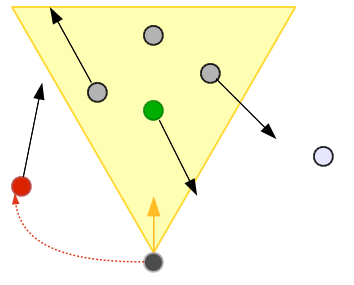
\includegraphics[scale=0.45]{./Ressources/Images/prefetchav.png}
        \caption{Exemple de gain possible pour le prefetching}
        \label{prefetchav}
        \end{figure}

\newpage


\newpage
\newpage
\section{Les autres améliorations possibles}

Une partie du stage a été de rechercher comment il serait possible de faire évoluer le travail réalisé dans Blue Banana. Nous allons donc présenter les différentes autres pistes que nous avons trouvé. La première solution consiste à se servir des déplacements en groupe des avatars. Une présentation rapide de ces mouvements de groupes permettra de mieux comprendre en quoi la piste d'amélioration peut être intéressante. Nous verrons ensuite un mécanisme de connaissance des routes entre les Hotspots, car actuellement les avatars se déplacent de façon aléatoire entre les Hotspots. Dans les jeux vidéos, les joueurs utilisent souvent les mêmes routes pour se déplacer. Cette piste permettrait de rendre les simulations et les solutions plus adaptées aux comportements des joueurs dans les MMOG.

\subsection{Les déplacements en groupes}

Dans cette partie, nous allons présentez les déplacements en groupe des avatars dans les MMOG. Cette étude permet de voir les avantages et les inconvénients de cette piste dans l'optique d'une amélioration du travail Blue Banana~\cite{191}. Le jeux en groupe (guilde et communauté) est une part importante de l'expérience que le joueur recherche en jouant à des MMOG~\cite{1501834,1255052}. Sans rentrer dans des détails sur la vie sociale \textit{réelle} des joueurs, nous allons étudier les comportements sociaux des joueurs. Ceci nous permettra de définir si la définition d'un modèle de mobilité et des améliorations de la réactivité sont possibles. Des études ont déjà démontré que des mouvement groupés existaient dans World of Warcraft~\cite{15141312}. La coopération est un facteur essentiel pour avoir le plus de réussite  dans les différentes missions proposées par le jeu. Un groupe de joueur permet de retrouver des personnes différentes et complémentaires, ce qui rend le groupe plus fort. Certains comparent même le fonctionnent des guildes au fonctionnement d'une \textit{famille de la mafia}~\cite{Jakobsson03thesopranos}.


%\newpage
\subsubsection{Étude des habitudes des joueurs de MMOG}
Nous allons étudier les différentes habitudes des joueurs de MMOG, et nous nous concentrerons sur les aspects sociaux du jeu, et avant tout sur les dynamiques de groupe présentes. Nous allons donner les points importants de deux études~\cite{1255052,StudyEQ}.


Griffiths, Davies et Chappell~\cite{BreakingSteretype} ont trouvé que l'aspect favori de 41\% des joueurs, est l'interaction sociale. De même Yee~\cite{1159988} a trouvé que 39,4\% des hommes et 53,3\% des femmes pensent que leurs amis \textit{dans le jeu} sont comparables à leurs amis dans la \textit{vie réelle}.
\par Certaines études~\cite{1124834,1031667} nous expliquent que les joueurs préfèrent en général jouer seul, d'autres~\cite{1159988,Jakobsson03thesopranos} insistent sur l'aspect \textit{social} que les joueurs recherchent dans ce genre de jeux vidéo. Nous pouvons donc dire que tous sont d'accord sur le fait que les interactions sociales sont courantes, et sont donc un facteur important des MMOG.
\par Les liens sociaux entre les joueurs ressemblent à des interactions dans le monde \textit{réel}, avec des comportements d'adhésion que l'on peut comparer aux mariages, avec des échanges commerciaux et même des \textit{services d'église}. Des normes sociales sont aussi présentes dans le jeu en plus des règles mises en place par l'éditeur (jargons, abréviations, émoticones, etc).

Dans~\cite{StudyEQ}, l'auteur a réalisé une étude sur les habitudes des joueurs de EverQuest. Environ 85\%, des personnes interrogées, nous disent qu'elles prennent plaisir à avoir des relations sociales dans le jeu. A la question: \textit{en quoi ils retirent le plus de satisfaction?}, la réponse \textit{se faire des amis} arrive dans le trio de tête ou aux portes de celui-ci (en fonction des hommes ou des femmes) très peu derrière gagner un niveau, réussir une quête et pillage d'un objet rare.
\par De plus, les personnes interrogées pensent à 50\% que leur amis de EverQuest sont comparables à ceux de leur vie "réelle". Lorsque les joueurs jouent en groupe, ils le font la majorité du temps avec des gens qu'il connaissent déjà (moins de 10\% avec des inconnus). Plus de 50\% de sondés sont très contents d'être dans leur guilde. Nous pouvons voir sur la figure~\ref{guildpres}, la participation des joueurs aux évènements de la guilde.
        \begin{figure}[!h]
        \centering
        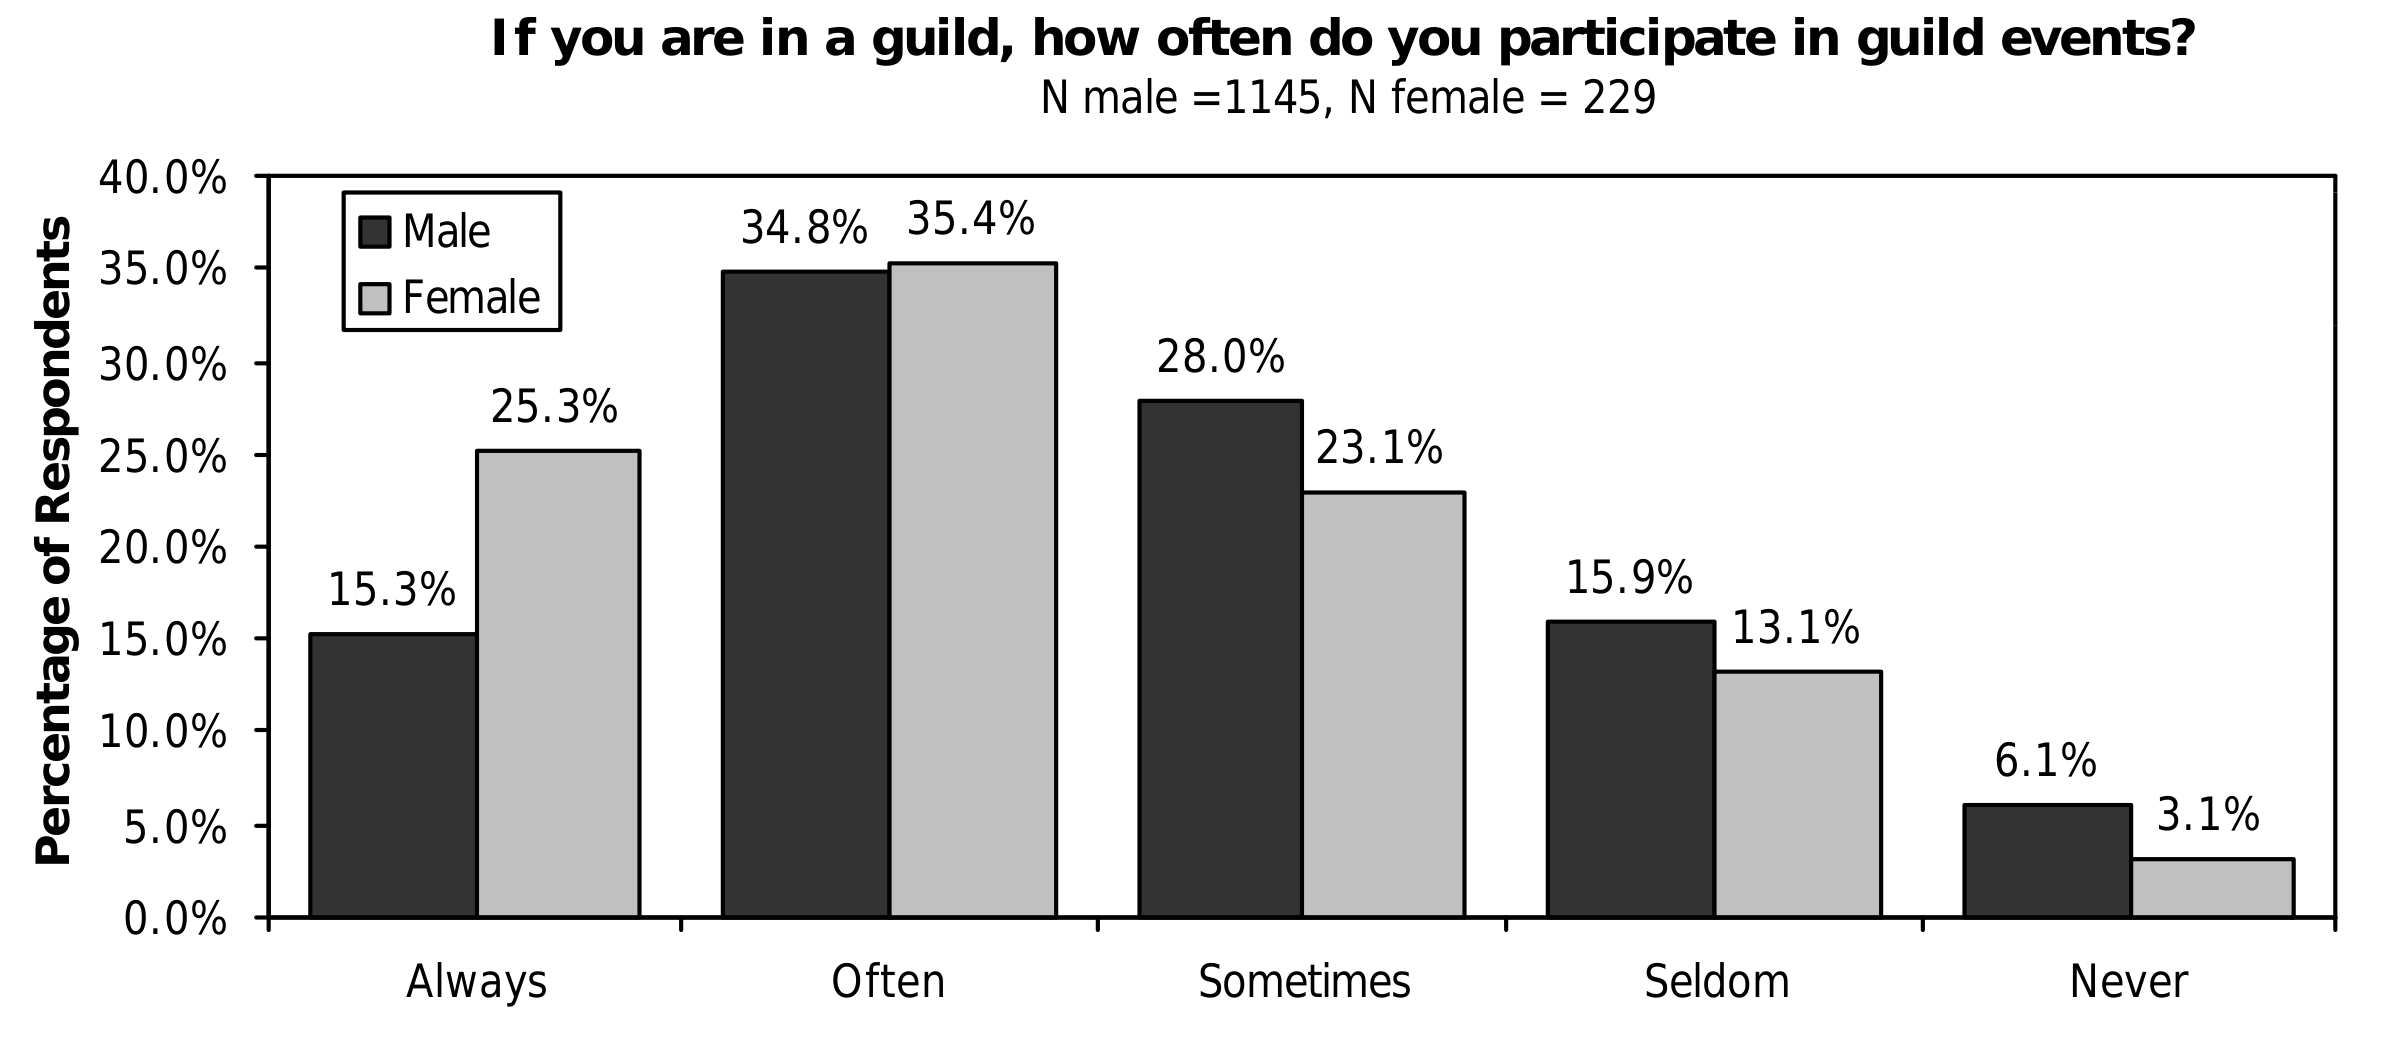
\includegraphics[scale=0.75]{./Ressources/Images/studypres.png}
        \caption{Participation des joueurs aux évènements de la guilde}
        \label{guildpres}
        \end{figure}

Cette étude donne des résultats qui sont, en grande majorité, similaires à l'étude précédente. Lorsque l'on demande aux joueurs quel est leur aspect préféré du jeu, l'aspect sociale se retrouve en deuxième position avec 23\% (1° place: 26\% pour passer des niveaux et faire évoluer son avatar) et même en première place, avec plus d'un tiers des suffrages, si l'on ajoute l'activité de chat et le \textit{role-playing} (23 + 10 + 5 = 38). L'article distingue trois types de joueurs: ceux qui se groupent pour jouer (34\%), ceux qui jouent pour se retrouver en groupe (55\%) et ceux qui ne se groupent pas (12\%).



\subsubsection{Les MMOG, des jeux socialisant?}
\par Dans~\cite{1124834}, les auteurs se sont intéressés aux dynamiques sociales dans les MMOG, et particulièrement dans le jeu World Of Warcraft~\cite{wow}. Unes des premières observations est que les joueurs vont jouer différemment en fonction de leur niveau. Par exemple, les joueurs vont passer moins de temps au niveau 39, car à partir du niveau 40 les joueurs pourront se déplacer plus rapidement dans le monde virtuel (60\%). Dans World Of Warcraft, 15\% des avatars sont au niveau 60, c'est à dire au niveau maximum.

\par Il est possible de remarquer que le temps passé en groupe évolue en fonction du niveau du joueur (voir figure~\ref{timespentgroup} ). Nous pouvons voir que le pourcentage de temps passé en groupe évolue en même temps que le niveau du joueur, pour se stabiliser à environ 40\%, et à partir du niveau 59 les joueurs passent plus de 50\% du temps en groupe. Les auteurs nous disent que les joueurs, qui ne font pas parti d'un groupe, vont évoluer de niveau plus rapidement. Ces joueurs rejoignent la plupart du temps des groupes lorsqu'ils ont atteint le niveau 55. 
	\begin{figure}[!h]
        \centering
        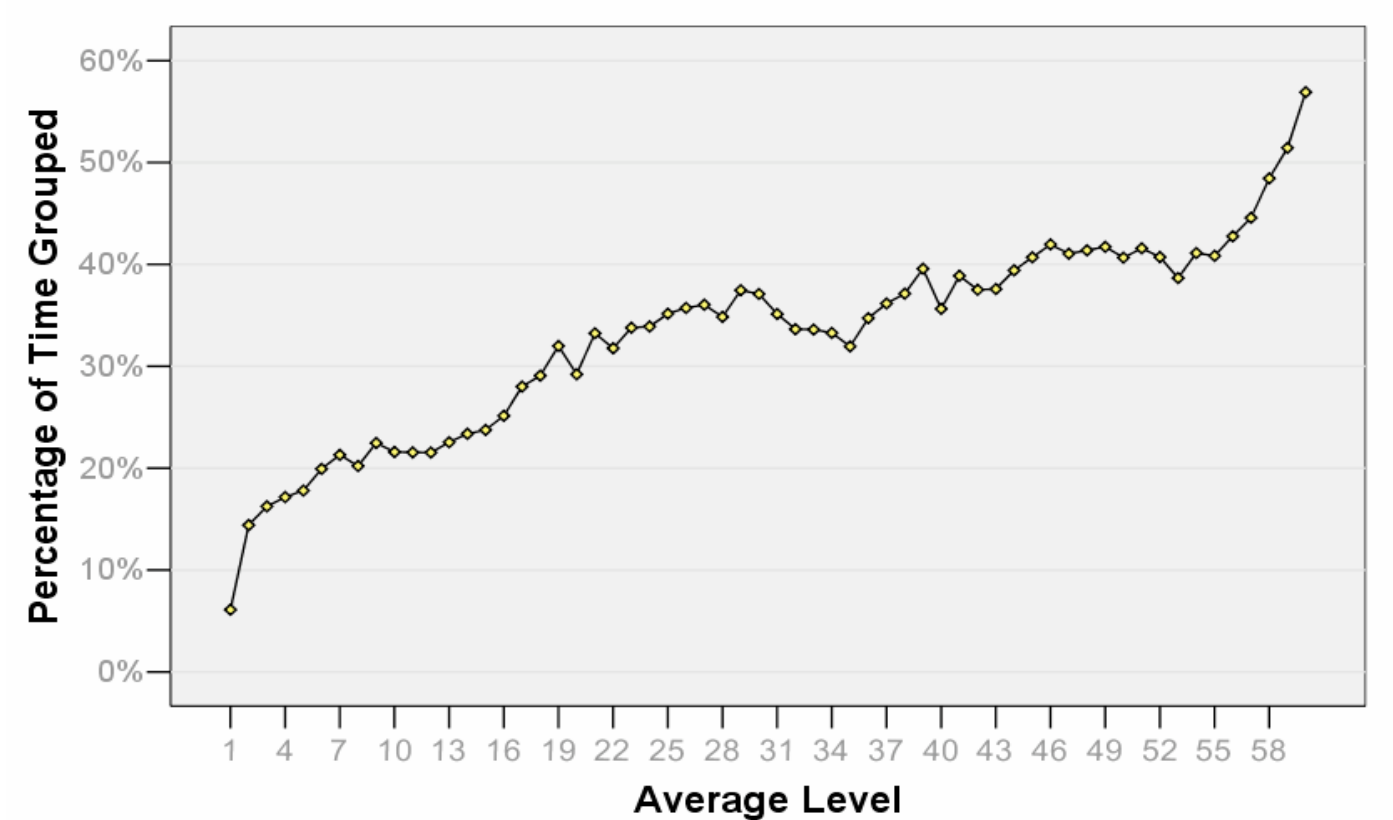
\includegraphics[scale=0.95]{./Ressources/Images/timespentgroup.png}
        \caption{Temps moyen passé en groupe, par niveau}
        \label{timespentgroup}
        \end{figure}

\par World Of Warcraft encourage les joueurs à former des groupes en utilisant deux mécanismes. Premièrement, pour qu'une complémentarité entre les habilitées des joueurs se crée. Deuxièmement, beaucoup de quêtes dans le jeu sont difficiles à réaliser tout seul. Nous pouvons aussi voir que des différences se dégagent entre le temps passé en groupe en fonction de chaque espèce (voir figure~\ref{tabltimegroup}).
\par Ces groupes sont appelés des guildes, elles sont un des aspects de la popularité de ce type de jeu. Dans World Of Warcraft, 66\% des avatars appartiennent à une guilde et ce chiffre atteint 90\% si l'on tient compte des joueurs ayant au moins le niveau 43. Les joueurs appartenant à une guilde joue en moyenne plus souvent qu'un joueur sans guilde. 
	\begin{figure}[!h]
        \centering
        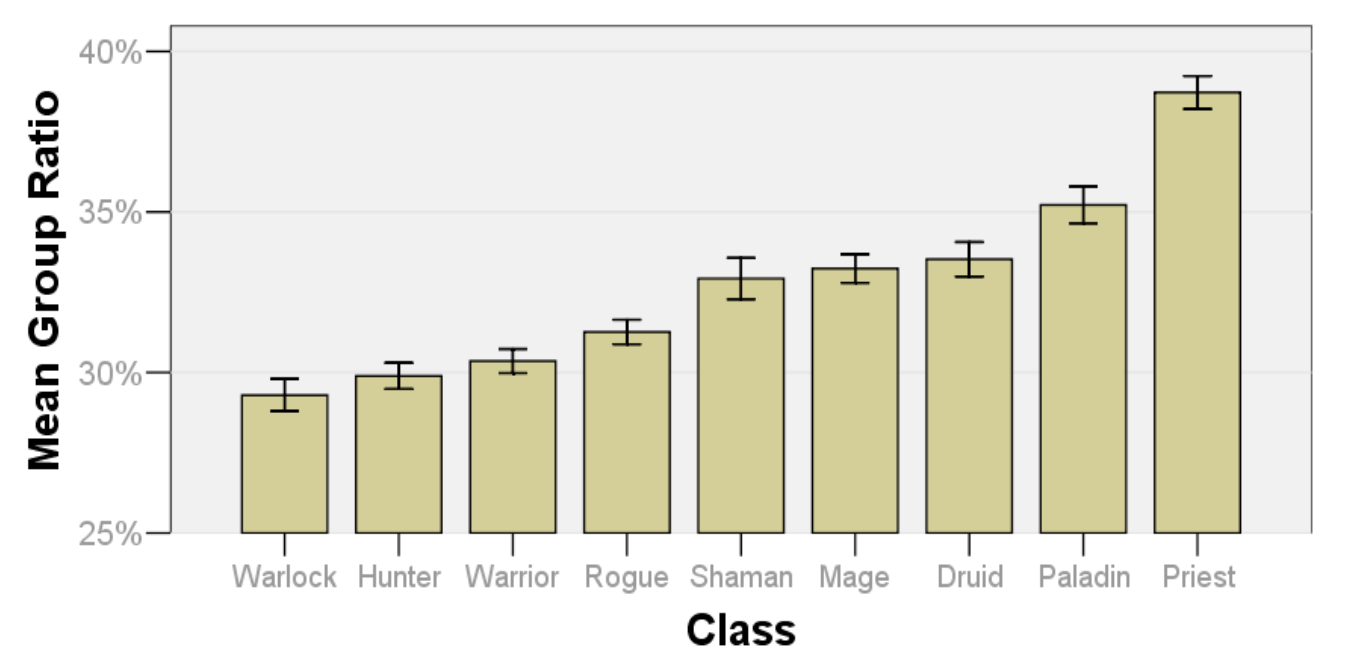
\includegraphics[scale=0.95]{./Ressources/Images/tabltimegroup.png}
        \caption{Temps moyen passé en groupe, par classe}
        \label{tabltimegroup}
        \end{figure}
\par Un des facteurs important, pour essayer de réaliser un modèle de mobilité, est d'étudier la taille des guildes. La moyenne de personne dans une guilde est de 14,5 (16,8 si l'on exclut du calcul les guildes d'une personne). Le median est de 6 (9 si l'on exclut du calcul les guildes d'une personne). 

\par Les auteurs ont mis en place un réseau social pour évaluer au mieux les guildes. Ils ont mis en place ce réseau selon deux méthodes différentes:
\begin{itemize}
	\renewcommand{\labelitemi}{$\bullet$}
	\item Une pour évaluer \textit{le potentiel de sociabilité des guildes:}\\
	Les joueurs sont connectés chacun aux autres (si en ligne au même moment),et cela sans tenir compte de leur localisation dans le jeu. Le réseau résultant reflète le spectre des opportunités des interactions sociales dans une guilde. Il va créer des liens entre les joueurs qui pourraient utiliser le "guild channel" et ceux qui font parti de la même guilde.
	\item Une pour quantifier \textit{les activités communes:}\\
	Les joueurs qui sont dans la même zone vont se connecter ensemble, sauf dans les grandes villes (Hotspots). Cette méthode permet de mettre en évidence les joueurs qui passent du temps ensemble, et qui se groupent en guilde pour exécuter des quêtes. Ces liens sont forts, car ils reflètent un intérêt mutuel. 
\end{itemize}

\par Les résultats montrent que les joueurs ne connaissent pas tous les joueurs du même guilde, et cela est d'autant plus vrai que le nombre de personnes, dans la guilde, est important. Des sous groupes peuvent aussi apparaître dans les guildes, surtout pour les guildes avec un nombre de joueurs important. 
\par Dans la figure~\ref{co-location}, il est possible de voir à quoi ressemble les liens entre les différents joueurs d'une même guilde de 41 membres. Tout d'abord 17 membres de la guilde n'ont jamais été observés dans la même zone qu'un autre membre. Un noyau central se distingue, il est composé de 8 joueurs qui jouent souvent ensemble, 3 autres joueurs forment un trio central où les liens épais montrent qu'ils passent beaucoup de temps ensemble. Les autres joueurs jouent avec 2 (ou moins) membres de la guilde.
	 \begin{figure}[!h]
        \centering
        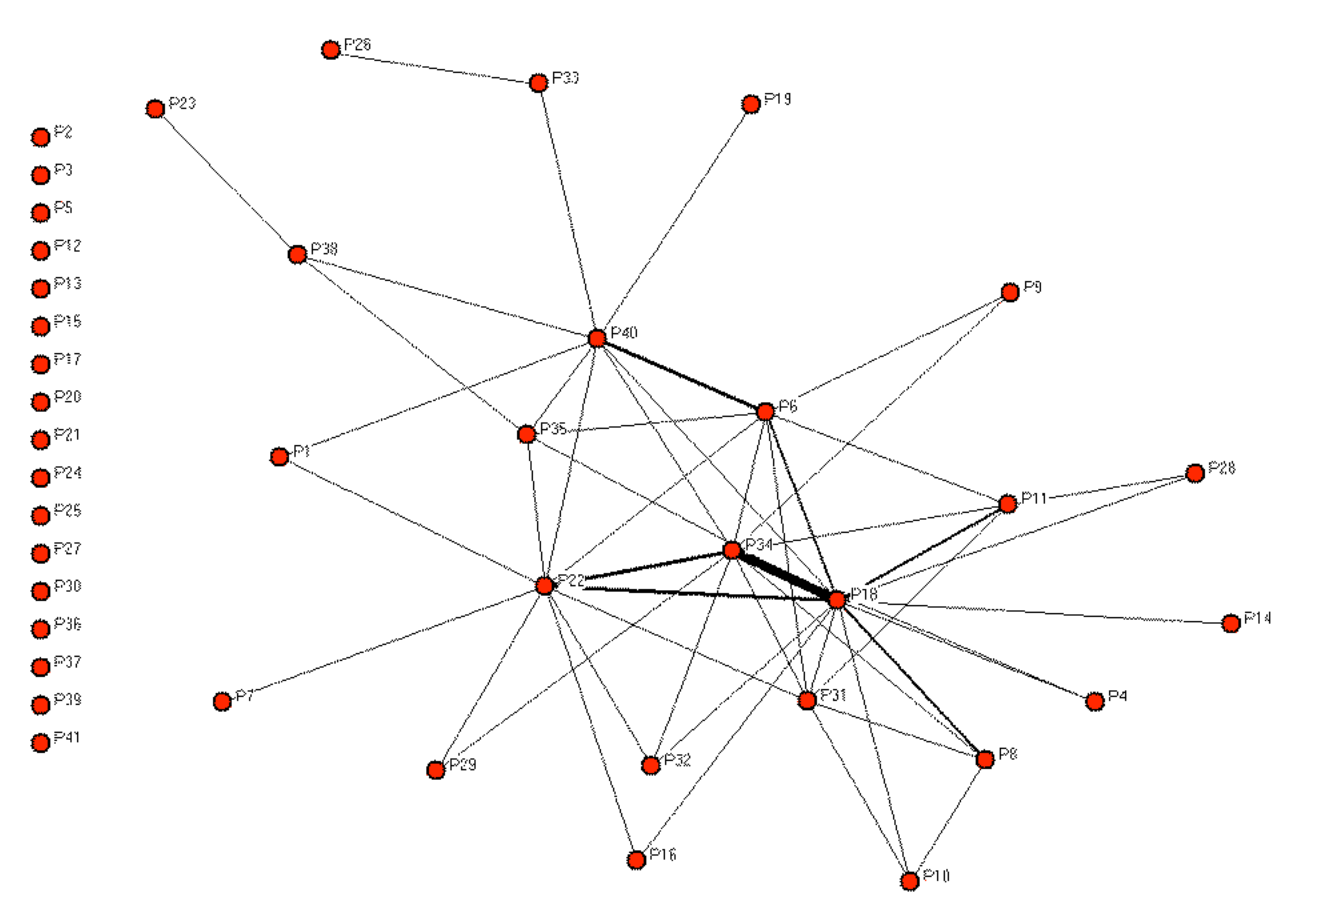
\includegraphics[scale=0.95]{./Ressources/Images/co-location.png}
        \caption{Co-location network dans une guilde de taille moyenne}
        \label{co-location}
        \end{figure}
%\newpage

%\section{The Sopranos Meets EverQuest}
%La coopération est un facteur essentiel pour avoir le plus de succès dans les différentes missions proposées par le jeu. Un groupe permet de retrouver des personnes différentes et complémentaires, ce qui rend le groupe plus fort. Certains comparent même le fonctionnent des guildes au fonctionnement d'une "famille de la mafia"~\cite{Jakobsson03thesopranos}.
\subsubsection{Conclusion sur l'étude des mouvements}
Nous avons pu remarquer que l'aspect communautaires des MMOG est un des points les plus importants pour les joueurs (voir figure~\ref{recapstat}). De plus, la majorité des études nous disent que la plupart des joueurs jouent en groupe pendant un temps non négligeable. Ces mouvements de groupe pourraient nous permettre de faire évoluer le module de prefetching, en formant des groupes où seulement certaines entités feraient du prefecting et les voisins des entités pourraient rester les mêmes.
\par Cette solution engendrerait de refaire le système de mobilité pour simuler des mouvements de groupe. Il faut aussi savoir que ces études sur les mouvements de groupe sont réalisées sur certains jeux~\cite{wow,everquest}. Ces mouvements de groupe n'existent pas ou sont moins perceptibles dans d'autres jeux~\cite{sl}. Il faudrait aussi mettre en place un système d'équilibrage des requêtes lors de mouvements de groupe, sinon certains travailleront toujours pour les autres.

	\vspace{5cm}
	\begin{figure}[!h]
        \centering
        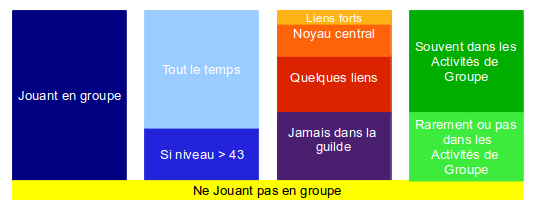
\includegraphics[scale=0.65]{./Ressources/Images/recapstat.png}
        \caption{Schéma récapitulatif des activités de groupe}
        \label{recapstat}
        \end{figure}

\subsubsection{Solution d'utilisation des mouvements de groupes}
\par L'utilisation des mouvements de groupe pourraient nous permettre de réorganiser le prefetching des données, et ne plus considérer les nœuds indépendamment mais comme formant un groupe. Ces groupes vont devoir avoir une organisation flexible et efficace. Les nœuds se trouvant en avant du groupe, selon la direction, pourrait être les seuls à rapatrier des données, ainsi nous économiserions des messages. Il faudrait ensuite transmettre les données vers les autres membres du groupe, plusieurs méthodes de diffusion peuvent être mises en place. La formation du groupe pourrait aussi permettre de mettre entre parenthèse la recherche de voisins (pour certains des nœuds en tout cas). 
\par La figure~\ref{mouvgroup} montre un exemple de ce à quoi pourrait ressembler la solution. Les nœuds, en gris foncé, vont rapatrier les données qui peuvent être intéressantes. Les autres nœuds du groupe n'auront pas rapatrier les données, mais il faudra ensuite diffuser ces données vers le reste du groupe.

	\vspace{1cm}
        \begin{figure}[!h]
        \centering
        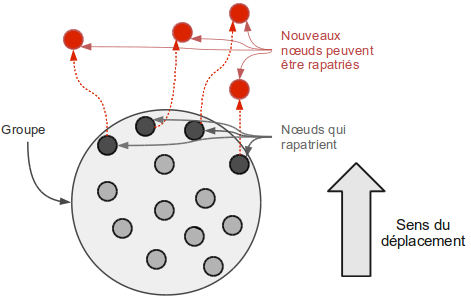
\includegraphics[scale=0.65]{./Ressources/Images/mouvgroup.png}
        \caption{Une piste pour les déplacements en groupe}
        \label{mouvgroup}
        \end{figure}

\newpage
 
\subsection{Mécanismes de connaissance des routes entre les Hotspots}
Dans cette solution, nous voudrions permettre aux avatars de suivre des routes, pour le contournement d'un obstacle par exemple. Il faudrait modifier le modèle pour ajouter des obstacles dans l'environnement. Deux solutions apparaissent rapidement pour créer ses routes. La première solution serait de définir des chemins pour contourner les obstacles, et de conserver ces chemins dans l'environnement. La deuxième solution consisterait à mettre en place un mécanisme d'apprentissage des routes par les avatars. Les avatars pourraient apprendre les routes au fur et à mesure des passages, et laisser des indications pour les avatars suivants. Cette solution permettrait de simuler un comportement réel, et ainsi d'essayer d'améliorer cette situation.
\par Les modifications sur le modèle ne seront peut être pas très simples à mettre en place. Il faudrait aléatoirement, comme il a été fait pour les Hotspots, définir des zones où les avatars ne pourraient pas passer ou seraient ralentis. Sur la figure~\ref{trajobstacle}, nous pouvons voir des trajectoires permettant d'éviter l'obstacle. Il faut définir si ces trajectoires se font par apprentissage ou si elles sont données avec l'initialisation de la carte.

	\begin{figure}[!h]
        \centering
        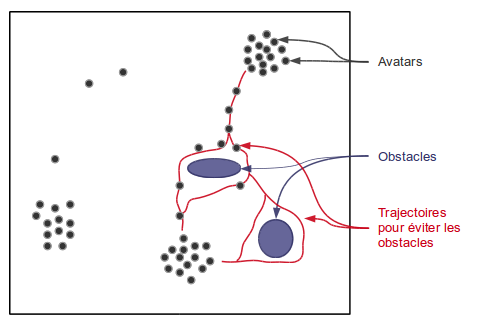
\includegraphics[scale=0.55]{./Ressources/Images/trajobstacle}
        \caption{Exemple de trajectoire d'évitement d'un obstacle}
        \label{trajobstacle}
	\end{figure}


\newpage
\subsection{Autres}
Dans cette partie, nous allons faire le tour d'autres idées d'amélioration, mais sans rentrer dans les détails comme nous avons pu le faire pour les autres. Des nœuds pourraient partager des liens encore plus forts que ceux du voisinage. Si deux nœuds vont dans la même direction et qu'ils ne sont pas trop éloignés (pas obligatoirement parmi les voisins), alors un lien pourrait se créer pour échanger des données.

\par Une autre amélioration pourrait être d'insérer des nœuds qui seraient fixe dans l'environnement, ils pourraient servir de "relais" dans certaines zones. Ces nœuds pourraient avoir plusieurs utilisations, nous pouvons imaginer qu'il pourrait servir de référent dans sa zone, ce mécanisme reviendrait à mixer un peu les solutions client/serveur et pair à pair. (FLOU)

\par Possibilité de créer des liens entre des nœuds qui sont proches dans le réseau. Ainsi deux nœuds qui sont proches pourrait échanger des données rapidement et ces données pourrait servir au nœud ultérieurement ou il pourrait les faire partager à d'autres nœuds sur le réseau virtuel. 
 
\par De la même façon que l'idée d'instaurer un cache, les nœuds pourrait se souvenir, en fonction de la zone géographique où ils se trouvent, d'anciens nœuds déjà rencontrés et ainsi tenter de communiquer avec eux prioritairement. (Trop Comme Cache)





\newpage
\section{Conclusion}
	Dans ce document, nous avons étudié différents mécanismes permettant d'améliorer la réactivité dans les applications pair à pair, et plus précisément dans les MMOGs. La nécessité d'amélioration des environnements virtuels ayant une architecture pair à pair est dû aux limitations de l'architecture client/serveur utilisée jusqu'à maintenant. Nous décrivons les différents mécanismes qui ont inspiré Blue Banana, qu'il faudra améliorer dans la suite du stage.\\
	Les mécanismes d'anticipation des mouvements donnent des résultats satisfaisants mais il sera nécessaire de trouver des améliorations pour mieux anticiper les mouvements en essayant de ne pas handicaper les performances de l'application.

	pheromones, mouvement des avatars en groupe, laisser des traces ( temporaire) des passages sur un nœud. Observations des déplacements des joueurs en équipe dans WOW.
		Signaler les points d'intérêt en dehors de l'AOI ? 
		Liens entre les avatars d'un même groupe.	
		



\newpage
\bibliographystyle{plain}
\bibliography{Biblio}


 

\end{document}

